\chapter{概率论基础}\label{chap:prob}

本附录主要介绍Kolmogorov概率论,讨论只局限在数学层面,不涉及概率论的哲学讨论. 本附录的连续型随机变量(向量)的讨论需要微积分的基本知识,关于微分学的部分,可以参见\Cref{chap:calculus};积分学(主要是Lebesgue积分)我们会在\Cref{sec:expectation} 以数学期望的形式介绍. 

\section{从朴素概率论到公理化概率论}

\subsection{Kolmogorov概率论}\label{subsec:kolmogorov-probability}
朴素的概率论通常讨论两种极端的情况,一个是可以用数数的方式来计算概率的情况,比如说掷骰子,另一个是用面积的方式来计算概率的情况,比如在随机选一个圆周上的点. 这两个情况分别对应了\emph{古典概型}和\emph{几何概型}. 

我们先给一些术语. 考虑一个随机试验,它的所有可能结果组成的集合称为\textbf{样本空间}\index{样本空间},记为$\Omega$. 样本空间的元素称为\textbf{样本点}\index{样本点},通常记为$\omega$. 样本空间的\emph{某些}子集被称为\textbf{事件}. 我们来看看这些概念在朴素的概率论中都具体是什么. 

\begin{example}[古典概型]
先后掷两个骰子,样本空间为
\[
    \Omega = \{ (i, j): 1 \leq i, j \leq 6 \}.
\]

样本点$(i, j)$表示第一个骰子掷出$i$点,第二个骰子掷出$j$点. 

“第一个骰子掷出$i$点”这个事件可以表示为$A_i = \{ (i, j): 1 \leq j \leq 6 \}$. “第一个骰子掷出$i$点,第二个骰子掷出$j$点”这个事件可以表示为$B_{ij} = \{ (i, j) \}$.
\end{example}

\begin{example}[几何概型]
在圆周上随机选点. 如果用弧度来表示圆周上的点,那么样本空间为
\[
    \Omega = [0, 2\pi).
\]

样本点为$\omega$,表示选出点的弧度. 

事件$A = [0, \pi)$表示选出了上半圆周,事件$B = [0, \pi/2)\cup[\pi, 3\pi/2)$表示选出了右上或左下的$1/4$圆周. 
\end{example}

那么,如何定义概率呢?朴素地说,概率是某个事件出现的可能性占总可能的比例. 

对于古典概型,我们简单认为每个样本点出现的概率都是相同的,也就是说,如果用$p_\omega$表示样本点$\omega$出现的概率,那么对任意$\omega\in\Omega$,都有$p_\omega = 1/|\Omega|$. 于是,对于任意事件$A$,它发生的概率为
\[
    \sum_{\omega\in A} p_\omega = \frac{|A|}{|\Omega|}.
\]
例如在上面掷骰子的例子中,$p_\omega=1/36$,$A$发生的概率为$1/6$,$B$发生的概率为$1/36$.

对于几何概型,不能再用古典概型的方式定义概率. 一段长为$2\pi$的圆弧上,有不可数个点. 如果选到每个点的概率相等,那么这个概率必须是$0$,否则所有点的概率和是无穷大. 更麻烦的是,我们也不能用古典概型的方式计算某个事件的概率!例如,选到上半圆周的概率,就是把所有上半圆周上的点的概率加起来,任意多个$0$相加依然还是$0$,所以这样的定义出来的概率永远是零,这样是不可行的. 

朴素的直觉告诉我们,选到上半圆周的概率是$1/2$,因为上半圆周刚好占了半个圆周. 所以几何概型的概率定义利用了\emph{体积}的概念. 事件$A$的概率定义为
\[
    \frac{\text{事件$A$对应的体积}}{\text{样本空间$\Omega$对应的体积}}.
\]
这里体积是广义上的,一维集合的体积就是长度,二维集合的体积就是面积,三维集合的体积就是体积,以此类推. 

例如在上面圆周的例子中,$A$对应的体积(长度)为$\pi$,$\Omega$对应的体积(长度)为$2\pi$,所以$A$发生的概率为$1/2$. 同理,$B$的概率也是$1/2$.

几何概型的定义看似合理,却并不严谨:我们并不知道如何定义“体积”. 我们来看一个有趣的例子. 

\begin{example}[Bertrand悖论]\index{Bertrand悖论}
考虑一个圆,它的半径为$1$. 现在我们随机地在圆上取一个弦,那么这个弦的长度超过$\sqrt{3}$(即圆内接正三角形的边长)的概率是多少?

我们给出三种答案,这三种答案对应了我们对“随机”的不同理解.

\begin{enumerate}[label=\textbf{解答\arabic*.},fullwidth,itemindent=2em]
    \item 不妨固定弦的其中一个点$A$,另一个点$B$在圆上等可能选取. 以$A$为顶点作圆内接正三角形$ACD$,弦的长度超过$\sqrt{3}$等价于$B$在弧$CD$上,所以概率为$1/3$.
    \item 弦长只与它到圆心的距离有关系,与方向无关. 弦长超过$\sqrt{3}$等价于它到圆心的距离小于$1/2$,所以概率为$1/2$.
    \item 弦被它的中点唯一确定,弦长大于$\sqrt{3}$等价于中点落在一个半径为$1/2$的同心小圆内,所以概率为同心小圆面积比上大圆面积,即$(1/2)^2=1/4$.
\end{enumerate}
三种解答的示意图见下(从左到右分别是解答1到3):
\begin{center}
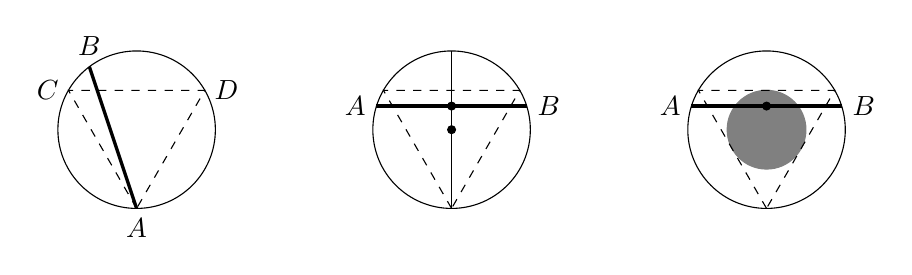
\begin{tikzpicture}
\draw (0,0) circle [radius=1];
\draw[dashed] (0,-1) node[below] {$A$} -- ({-sqrt(3)/2},0.5) node[left] {$C$} -- ({sqrt(3)/2},0.5) node[right] {$D$} -- cycle;
\draw[very thick] (0,-1) -- (-0.6,0.8) node[above] {$B$};

\draw (4,0) circle [radius=1];
\draw (4,-1) -- (4,1);
\draw[dashed] (4,-1)-- ({4-sqrt(3)/2},0.5)  -- ({4+sqrt(3)/2},0.5) -- cycle;
\draw[fill] (4,0) circle [radius=0.05];
\draw[fill] (4,0.3) circle [radius=0.05];
\draw[very thick] ({4-sqrt(1-0.3^2)},0.3) node[left] {$A$} -- ({4+sqrt(1-0.3^2)},0.3) node[right] {$B$};

\draw (8,0) circle [radius=1];
\draw[fill,gray] (8,0) circle [radius=0.5];
\draw[dashed] (8,-1)-- ({8-sqrt(3)/2},0.5)  -- ({8+sqrt(3)/2},0.5) -- cycle;
\draw[fill] (8,0.3) circle [radius=0.05];
\draw[very thick] ({8-sqrt(1-0.3^2)},0.3) node[left] {$A$} -- ({8+sqrt(1-0.3^2)},0.3) node[right] {$B$};
\end{tikzpicture}
\end{center}
\end{example}

同样的事件因为我们对“随机”的理解不同,得到了不同的概率!因此,我们需要一个更加严格的定义来描述概率. 

首先注意到,概率应该是一个函数,它的值域是$[0,1]$. 那么,它的定义域应该是什么呢?我们已经看到,概率应该定义在\emph{事件}上,而非\emph{样本点}上. 那么,概率可以定义在\emph{任意}事件上吗?这个问题很微妙,我们不在这里讨论. 这里只是指出,我们关心的并不总是任意事件,而是一类被$\sigma$-代数所刻画的事件. 

\begin{definition}[$\sigma$-代数]\index{$\sigma$-代数}
设$\Omega$是一个集合,$\scF$是$\Omega$的子集的集合. 如果$\scF$满足
\begin{enumerate}
    \item $\Omega\in\scF$;
    \item 如果$A\in\scF$,则$A$的补集$\Omega\setminus A\in\scF$;
    \item 如果$A_1,A_2,\ldots\in\scF$,则$\bigcup_{i=1}^\infty A_i\in\scF$.
\end{enumerate}
则称$\scF$是$\Omega$上的一个 \textbf{$\sigma$-代数}. 
\end{definition}


在样本空间中,我们要求事件也形成一个$\sigma$-代数,这样的$\sigma$-代数称为\textbf{事件域}\index{事件域},记为$\scF$. 在数学上,$\sigma$-代数包括了绝大部分我们可以构造的事件,这是因为,容易验证,$\sigma$-代数中的事件对可数交、可数并和补运算都是封闭的,并且包含了样本空间和空集. 关于这一定义的哲学讨论,可以见\Cref{chap:plausible-reasoning}.  

样本空间连同它的事件域,被称为\emph{可测空间}. 

\begin{definition}[可测空间] \index{可测空间}
设$\Omega$是一个集合,$\scF$是$\Omega$上的一个$\sigma$-代数. 则称$(\Omega,\scF)$是一个\textbf{可测空间}.

设$S\subseteq\Omega$,如果$S\in\scF$,则称$S$是\textbf{$\scF$-可测}的.
\end{definition}

定义可测空间与$\scF$-可测的概念,主要是为了区分一个集合到底是不是我们所关心的事件,我们只关心$\scF$-可测的集合.

接下来,我们给出Kolmogorov概率论的公理化定义. 

\begin{definition}[概率空间,概率测度]\index{概率空间}\index{概率}\index{概率测度}
设$(\Omega,\scF)$是一个可测空间. 如果函数$\Pr:\scF\to[0,1]$满足
\begin{enumerate}
    \item 正则性:$\Pr(\Omega)=1$;
    \item 可列可加性:如果$A_1,A_2,\dots\in\scF$是两两不相交的事件,则
    \[
        \Pr\left(\bigcup_{i=1}^\infty A_i\right) = \sum_{i=1}^\infty \Pr(A_i),
    \]
    则称$(\Omega,\scF,\Pr)$是一个\textbf{概率空间},$\Pr$称为\textbf{概率测度}或\textbf{概率}. 
\end{enumerate}
\end{definition}

容易证明,概率有如下性质:
\begin{proposition}
设$(\Omega,\scF,\Pr)$是一个概率空间,则:
\begin{enumerate}
    \item $\Pr(\varnothing)=0$;
    \item 单调性:对任意的$A,B\in\scF$,如果$A\subseteq B$,则$\Pr(A)\leq\Pr(B)$;
    \item 有限可加性:对两两不相交的$A_1,A_2,\dots,A_n\in\scF$,有
    \[
        \Pr\left(\bigcup_{i=1}^n A_i\right) = \sum_{i=1}^n \Pr(A_i).
    \]
\end{enumerate}
\end{proposition}

他们的证明都不困难,我们略去. 

下面,我们回到古典概型与几何概型,看看如何对他们构造概率空间.  

对于古典概型来说,我们容易写出它的概率空间. 此时事件域恰好为所有$\Omega$的子集的集合,概率测度的定义也就是我们之前的定义:$\Pr(A)=|A|/|\Omega|$. 

对于几何概型来说,概率空间最大的困难在于事件域和概率测度的定义. 为了简化讨论,我们集中在$\Omega=[0,1]^n$,也就是$n$维立方体的情况. 

先考虑事件域. 首先,事件域至少要包含长方体
\[\prod_i(a_i,b_i)=\{x=(x_1,x_2,\ldots,x_n)\in\R^n:a_i<x_i<b_i\}.\]
这是我们可以构造的最基本的集合了. 我们就定义事件域为包含所有长方体的最小$\sigma$-代数$\scB([0,1]^n)$. 换言之,如果还有一个$\sigma$-代数$\scF$包含所有长方体,那么$\scB([0,1]^n)\subseteq\scF$. 我们将这一$\sigma$-代数称为\textbf{Borel代数}\index{Borel代数}. Borel代数包含了绝大部分我们要讨论的集合,例如开集、闭集、单点集、有限集、可数集等,可以简单归纳为“合理的集合”. 

事件域的定义已经给出,我们还需要定义概率测度$\Pr$,它应该满足以下两个要求:
\begin{itemize}
    \item 让正方体的概率等于它的体积. 按照朴素的直觉,长方体$\prod_i(a_i,b_i)$的体积应该是$\prod_i(b_i-a_i)$,也就是
    \[
        \Pr\left(\prod_i(a_i,b_i)\right) = \prod_i(b_i-a_i).
    \]
    \item 平移不变性. 也就是说,如果$A\in\scB([0,1]^n)$,那么对任意的$x\in\R^n$,定义$A+x=\{y\in\R^n:y=x+z,z\in A\}$,只要$A\in\scB([0,1]^n)$,就有$\Pr(A+x)=\Pr(A)$.
\end{itemize}
一个惊人的事实是,这样的概率测度是存在且唯一的,我们称之为\textbf{Lebesgue测度}\index{Lebesgue测度},常记为$\lambda$.

注意,Borel代数和Lebesgue测度的定义可以不局限在$[0,1]^n$,他们可以定义在与实数相关的各种集合上. 在本附录中,我们最主要是用的是$\R^n$上的相关定义,例如$\scB(\R^n)$就是包含所有$n$维开长方体(每条边是开区间)的最小$\sigma$-代数,$\lambda$就是定义在$\scB(\R^n)$上的Lebesgue测度. $\R^n$上的Lebesgue测度其实是概率测度的扩展(而非概率测度),因为此时不再要求有正则性(即$\lambda(\Omega)=1$),但额外要求$\lambda(\varnothing)=0$.

\subsection{条件概率,独立性}
接下来,我们讨论条件概率与独立性. 我们还是看掷两个骰子的例子. 掷完第一个骰子,我们马上观察结果,然后再掷第二个骰子. 问第一个骰子是$i$,第二个是$j$的概率是多少?如果继续套用原来的概率空间,很快就会觉得不对劲. 此时,第一个骰子的结果完全没有随机性!所以朴素的直觉告诉我们,这里的概率应该有另一个依赖于第一次投骰子结果的定义,这样的概率就是\emph{条件概率}. 

我们直接给出一般情况下条件概率的定义. 

\begin{definition}[条件概率]\index{条件概率}
设$(\Omega,\scF,\Pr)$是一个概率空间,$A,B\in\scF$是两个事件,且$\Pr(A)>0$. 则称
\[
    \Pr(B|A) = \frac{\Pr(A\cap B)}{\Pr(A)}
\]
是事件$B$在事件$A$发生的条件下发生的\textbf{条件概率}. 
\end{definition}

以上定义要求$A$发生概率为正,然而,$A$是零概率的时候也是可能有条件概率的. 例如,
从$[0,1]\times[0,1]$中均匀地随机选一个点$(X,Y)$,观察它的横坐标$X$. 不管什么样的$x$,$X=x$的概率都是$0$. 然而,直觉上,条件在$X=x$上,$Y>1/2$的概率不仅存在,而且应该是$1/2$. 在\Cref{sec:random-variable} 中,我们会针对一类特殊的事件,给出此时条件概率的定义. 

我们继续看投两个骰子的例子. 假设事件$A$是“第一个骰子是$i$“,事件$B$是“第二个骰子是$j$”. 我们可以计算出$\Pr(B|A)=\Pr(B)=1/6$. 如果单看计算的结果,这是一个非常神奇的式子:条件在$A$上和不条件在$A$上概率是一样的!从直觉来说,这件事情却并不神秘,因为第一个骰子的结果和第二个骰子的结果是不应该有关系的. 我们把这种现象称为\textbf{独立性}. 更一般地,对任意事件$A,B$,如果$\Pr(A)>0$,那么
\[\Pr(B|A)=\Pr(B)\iff \frac{\Pr(A\cap B)}{\Pr(A)}=\Pr(B)\iff \Pr(A\cap B)=\Pr(A)\Pr(B).\]
最后一个式子并不要求$\Pr(A)>0$,因此我们用它作为独立性的定义,这样定义可以不依赖条件概率. 

\begin{definition}[独立性]\index{独立性}
设$(\Omega,\scF,\Pr)$是一个概率空间,$A,B\in\scF$是两个事件. 如果$\Pr(A\cap B)=\Pr(A)\Pr(B)$,则称事件$A$和$B$\textbf{相互独立}. 

一般地,给定一个事件族$\mathscr{A}\subseteq\scF$,如果对任意的有限个不同的$A_1,A_2,\ldots,A_n\in\mathscr{A}$,都有
\[
    \Pr\left(\bigcap_{i=1}^n A_i\right) = \prod_{i=1}^n \Pr(A_i),
\]
则称事件族$\mathscr{A}$中的事件是\textbf{相互独立}的. 
\end{definition}

我们在定义中还给出了多个事件相互独立的定义,这一定义是说不管挑出其中多少有限个事件,他们都应该满足交的概率等于概率的积. 这并\emph{不等价}于任意两个事件都相互独立,我们看下面的例子. 

\begin{example}
两个人进行石头剪刀布游戏,每个人独立等概率地出剪刀石头布. 

考虑下面三个事件:$A=\{\text{甲出了石头}\}$,$B=\{\text{乙出了剪刀}\}$,$C=\{\text{甲赢}\}$.

容易算出,$\Pr(A\cap B)=\Pr(A)\Pr(B)=1/9$,$\Pr(A\cap C)=\Pr(A)\Pr(C)=1/9$,$\Pr(B\cap C)=\Pr(B)\Pr(C)=1/9$,所以$A,B,C$两两独立. 

但是$A,B,C$不是相互独立的:$\Pr(A\cap B\cap C)=1/9\neq 1/27=\Pr(A)\Pr(B)\Pr(C)$.
\end{example}

这个例子说明,三个事件的独立性远比他们任意两个之间的独立性要复杂,三个事件放在一起可能才会出现不独立的情况. 对于一般情况,这样的现象更加普遍,所以我们多个事件的独立性定义是要求任意有限个事件都独立,而不是任意两个事件都独立. 

最后,我们给出条件概率的一些性质. 

\begin{proposition}\label{prop:conditional-probability}
设$(\Omega,\scF,\Pr)$是一个概率空间,那么
\begin{enumerate}
    \item 对任意$A\in\scF$满足$\Pr(A)>0$,$\Pr(\cdot|A)$也是一个概率测度;
    \item $\Pr(\cdot|\Omega)=\Pr(\cdot)$,
    \item 对任意$A\in\scF$满足$\Pr(A)>0$,$\Pr(A|A)=1$.
\end{enumerate}
\end{proposition}
以上性质的证明都很简单,我们就不给出了. 

接下来我们给两个在Bayes概率论\index{Bayes概率论}以及随机过程\index{随机过程}中很重要的性质. 

\begin{theorem}[全概率公式]\index{全概率公式}\label{thm:total-probability}
设$(\Omega,\scF,\Pr)$是一个概率空间,$A_1,A_2,\ldots\in\scF$是一列两两不相交的事件,且$\Pr(A_i)>0$,$\bigcup_{i=1}^\infty A_i=B$,则对任意的$C\in\scF$,有
\[
    \Pr(C|B) = \sum_{i=1}^\infty \Pr(C|A_i)\Pr(A_i).
\]
特别地,对于有限个$A_i$,这一定理也成立. 
\end{theorem}
\begin{proof}
注意到
\[
    \Pr(C) = \Pr(C\cap B) = \Pr\left(C\cap\bigcup_{i=1}^\infty A_i\right) = \Pr\left(\bigcup_{i=1}^\infty (C\cap A_i)\right) = \sum_{i=1}^\infty \Pr(C\cap A_i).
\]
最后一个等号是因为$C\cap A_i$两两不相交. 另一方面,
\[
    \Pr(C\cap A_i) = \Pr(C|A_i)\Pr(A_i),
\]
所以
\[
    \Pr(C) = \sum_{i=1}^\infty \Pr(C|A_i)\Pr(A_i).
\]
对于有限个$A_i$,只需要把无穷求和改成有限求和,利用有限可加性即可. 
\end{proof}

全概率公式是一种分而治之的思想,它把一个复杂的事件分解成若干个简单的事件,然后再把简单的事件的概率加起来. 我们来看一个例子. 

\begin{example}
    从装有$w$个白球和$b$个黑球的盒子中随机地取出一个球,不放回,再取出一个球. 问第二个球是白球的概率是多少?

    设事件$A$是“第一个球是白球”,事件$B$是“第二个球是白球”. 我们有
\begin{align*}
    \Pr(B) &= \Pr(B|A)\Pr(A) + \Pr(B|\bar{A})\Pr(\bar{A}) \\
    &=\frac{w-1}{w+b-1}\cdot\frac{w}{w+b} + \frac{w}{w+b-1}\cdot\frac{b}{w+b}\\
    &=\frac{w}{w+b}.
\end{align*}
    这里$\bar A$指的是$A$的补集,即“第一个球是黑球”. 
\end{example}

\begin{theorem}[贝叶斯公式]\index{贝叶斯公式}\label{thm:bayes}
设$(\Omega,\scF,\Pr)$是一个概率空间,$A,B\in\scF$且$\Pr(A),\Pr(B)>0$,则
\[
    \Pr(A|B) = \frac{\Pr(B|A)\Pr(A)}{\Pr(B)}.
\]
\end{theorem}

这一公式的证明几乎是显然的,我们略去. 

一个特别重要的推论被称为\emph{链式法则}\index{链式法则},它是\emph{Bayes网络}\index{Bayes网络}的基础. 

\begin{corollary}[链式法则]\index{链式法则}\label{cor:chain-rule}
设$(\Omega,\scF,\Pr)$是一个概率空间,$A_1,A_2,\ldots,A_n\in\scF$,且$\Pr(A_1\cap A_2\cap\cdots\cap A_n)>0$,则
\begin{align*}
    &\Pr(A_1\cap A_2\cap\cdots\cap A_n)\\
    = &\Pr(A_1)\Pr(A_2|A_1)\Pr(A_3|A_1\cap A_2)\cdots\Pr(A_n|A_1\cap A_2\cap\cdots\cap A_{n-1}).
\end{align*}
\end{corollary}

我们也看一个例子. 

\begin{example}[P\'olya的罐子]
    一个罐子装有$w$个白球和$b$个黑球,随机取出一个,观察它的颜色,放回,再放回相同颜色的$c$个球,再随机取一次,重复上述操作,如此反复$n$次,问每一次都取到白球的概率是多少?

    设事件$A_i$是“第$i$次取出的球是白球”. 我们有
\begin{align*}
    \Pr(A_1)&=\frac{w}{w+b},\\
    \Pr(A_2|A_1)&=\frac{w+c}{w+b+c},\\
    \Pr(A_3|A_1\cap A_2)&=\frac{w+2c}{w+b+2c},\\
    &\cdots\\
    \Pr(A_n|A_1\cap A_2\cap\cdots\cap A_{n-1})&=\frac{w+nc}{w+b+nc}.
\end{align*}
    所以
\[
    \Pr(A_1\cap A_2\cap\cdots\cap A_n) = \frac{w}{w+b}\cdot\frac{w+c}{w+b+c}\cdots\frac{w+nc}{w+b+nc}.
\]
\end{example}

\begin{remark}
    在概率论中,我们经常要讨论事件的交,所以我们通常会把$A\cap B$简记为$AB$. 此外,事件不相交我们也称之为\textbf{互斥}\index{互斥}. 事件$A$的补事件,即$\Omega\setminus A$.我们会记为$\bar{A}$或$A^c$.
    
    另外,我们也经常要讨论一个关于$\omega$的陈述$Q(\omega)$定义的事件$\{\omega\in\Omega:Q(\omega)\}$,在P\'olya的罐子的例子中,事件$A_1$其实就是由陈述$Q(\omega)$:“$\omega$中第一次取出的球是白球”定义的事件. 在这种情况下,我们将这一事件简记为$\{Q\}$,它的概率就是$\Pr(\{Q\})$或者简记为$\Pr(Q)$. 
    
    最后,事件交的概率也经常以逗号的形式写出. 例如,在P\'olya的罐子的例子中,我们会把概率$\Pr(A_1A_2)$记为
    \[\Pr(\text{第一次取出的球是白球},\text{第二次取出的球是白球}).\] 
    这样的记号更直观,并且在随机变量部分会经常使用. 
\end{remark}

\section{随机变量,分布函数}\label{sec:random-variable}

接下来,我们讨论随机变量. 从某种意义上说,随机变量是另一种刻画概率测度的手段. 不过,随机变量能够更加直观、定量描述概率空间中的事件,所以这是一个更加容易使用的概念. 

\subsection{基本定义}

为了理解随机变量的概念,我们依然从古典概型入手. 

\begin{example}\label{ex:random-variable}
继续考虑先后投两个骰子的情况,假设它的概率空间是$(\Omega,\scF,\Pr)$,他们的定义我们在\Cref{subsec:kolmogorov-probability} 的末尾已经讨论过了. 

我们可以定义一个从样本空间$\Omega$到$\N$的函数$S(i,j)=i+j$,也就是两个点数的和. 我们来看看$S$与事件域的关系. $\{S=s\}=\{(i,j)\in\Omega:i+j=s\}$,所以$S$将原本的事件精简成了一个数字. 这个过程丢弃了一些事件,例如$S$无法表达事件$\{(1,2)\}$,实际上,它无法区分$(1,2)$和$(2,1)$,它把这两个样本点都看成了$3$. 但是,$S$仍然保留了很多信息,例如,$S$可以区分事件$\{(1,1)\}$和$\{(2,2)\}$,它们分别对应$2$和$4$. 总结来说,$S$将原本更精细的事件域压缩成了更粗糙的事件域. 

有了上面的感觉,我们可以看一个更抽象的函数. 定义一个从样本空间$\Omega$到$\N^2$的函数$X$,它的定义为$X(i,j) = (i,j)$. 换句话说,它把样本点看成一个$\N^2$的元素. $\scF$中的所有事件都可以表达为$\{X\in B\}$,$B\subseteq\N^2$. 所以$X$完全刻画了整个事件域. 
\end{example}

上面例子中的$S$和$X$都是\emph{随机变量}的例子. 我们给出随机变量的定义. 

\begin{definition}[随机变量,随机向量,Borel函数]\index{随机变量}\index{随机向量}\index{Borel函数}
设$(\Omega,\scF,\Pr)$是一个概率空间,$X:\Omega\to\R$是一个函数. 如果对任意的$x\in\R$,$\{X\in\scB(\R)\}\in\scF$,则称$X$是一个\textbf{随机变量}. 

一般地,考虑一个集合$\R^n$以及其上的Borel代数$\scB(\R^n)$,$X:\Omega\to \R^n$是一个映射. 如果对任意的$A\in\scB(\R^n)$,集合$\{X\in A\}$ $\scF$-可测,即$\{X\in A\}\in\scF$,则称$X$是一个\textbf{$n$维随机向量},简称\textbf{随机向量}. 如果$(\Omega,\scF)=(\R^m,\scB(\R^m))$,则称$X$是一个\textbf{Borel函数}.
\end{definition}

下面对这个定义做一些说明. 首先,随机变量是一个映射,而不是一个数字,这一点经常会被人误解. 直观上说,随机变量的值是随机的,这个随机性是因为背后有一个未知的力量在抛硬币,我们把从抛硬币到观测值这一整个东西称之为随机变量. 

定义的后面还涉及了$\sigma$-代数相关的东西,我们也给一个简要说明. Borel代数包含了“合理的集合”,所以$\{X\in B\}$($B\in\scB(\R)$)表示事件“$X$落在合理的值集上”. 随机变量的要求其实就是,“$X$落在合理的值集上”是一个我们可以定义概率(即可测)的事件. 

我们下面讨论一些随机变量的基本性质. 

\begin{theorem}\label{thm:random-variable}
设$(\Omega,\scF,\Pr)$是一个概率空间,$X:\Omega\to\R^n$是一个随机向量,$g:\R^n\to\R^m$是一个Borel函数,则$g(X)=g\circ X$也是一个随机向量. 
\end{theorem}

这一性质告诉我们了一种构造随机变量的方式:对一个随机变量进行一些Borel函数的操作. 下面的性质告诉我们,Borel函数包含了绝大部分我们关心的函数,因此在实际中,我们不需要担心一个映射作用完之后是否还是随机变量.

\begin{proposition}\label{prop:borel-function}
下面函数是Borel函数:
\begin{enumerate}
    \item 所有的连续函数;
    \item 给定$A\in\scB(\R^n)$,示性函数\index{示性函数}
    $I_A(x) = \begin{cases}
        1, & x\in A,\\
        0, & x\notin A.
    \end{cases}$
    \item 两个Borel函数的复合函数. 
\end{enumerate}
\end{proposition}



接下来,我们进入分布函数的讨论. 我们说过,随机变量某种意义上给出了概率测度的另一种刻画方式,而这一桥梁就是由分布函数给出的. 

考虑概率空间$(\Omega,\scF,\Pr)$,以及一个随机变量$X:\Omega\to\R$. 要刻画概率测度$\Pr$,我们需要给出所有的事件$A\in\scF$的概率$\Pr(A)$. 如果$A$可以被写成$\{X\in B\}$的形式,那么我们可以用$\Pr(X\in B)$来刻画$\Pr(A)$. 而我们之前说过,要确定$\Pr(X\in B)$,至少要先确定$\Pr(X\in(a,b))$. 这一概率还是有两个未定元$a,b$,所以更简便的方式是确定$F_X(b)=\Pr(X\in(-\infty,b])$,容易证明,开区间的概率完全可以由$F_X(b)$给出,所以$F_X$完全刻画了$\Pr$. 更一般地,我们有如下定义. 

\begin{definition}[分布函数]\index{分布函数}
设$(\Omega,\scF,\Pr)$是一个概率空间,$X:\Omega\to\R$是一个随机变量. 定义函数$F_X:\R\to\R$为$F_X(x) = \Pr(X\leq x)$. 我们称$F_X$是$X$的\textbf{分布函数},记作$X\sim F_X$.

如果$X:\Omega\to\R^n$是一个随机向量,定义函数$F_X:\R^n\to\R$为$F_X(x) = \Pr(X\leq x)$,这里$X\leq x$是指对任意的$i=1,2,\ldots,n$,都有$X_i\leq x_i$. 我们称$F_X$是$X$的\textbf{分布函数},记作$X\sim F_X$.
\end{definition}

容易验证,分布函数具有如下的性质:

\begin{proposition}\label{prop:distribution-function}
设$(\Omega,\scF,\Pr)$是一个概率空间,$X:\Omega\to\R$是一个随机变量,$F_X$是它的分布函数,则
\begin{enumerate}
    \item $F_X$是一个非减函数;
    \item $\lim_{x\to-\infty}F_X(x)=0$,$\lim_{x\to+\infty}F_X(x)=1$;
    \item $F_X$是右连续的,即对任意$x\in\R$,都有$\lim_{y\downarrow x}F_X(y)=F_X(x)$;
    \item $F_X$在每一点处的左极限存在,即对任意$x\in\R$,都有$F(x-)=\lim_{y\uparrow x}F_X(y)$存在.
\end{enumerate}
\end{proposition}

实际上,分布函数也可以由\Cref{prop:distribution-function} 的前三条性质给出定义,这是因为,满足前三条性质的函数恰好是某个随机变量的分布函数:

\begin{theorem}\label{thm:distribution-function}
设$F$是$\R\to\R$的函数,满足\Cref{prop:distribution-function} 的前三条性质. 

在概率空间$([0,1],\scB([0,1]),\lambda)$上,存在一个随机变量$X$,使得$F_X=F$.
\end{theorem}

所以,我们今后也称呼满足\Cref{prop:distribution-function} 四条性质的函数为分布函数. 

我们看一个分布函数计算概率的简单例子. 
\begin{example}\label{ex:distribution-prob}
    考虑$\R$上的分布函数$F$,它由随机变量$X$定义. 那么,
    \begin{itemize}
        \item $\Pr(X\leq a)=F(a)$,
        \item $\Pr(X<a)=F(a-)$,
        \item $\Pr(X>a)=1-F(a)$,
        \item $\Pr(X\geq a)=1-F(a-)$,
        \item $\Pr(X=a)=F(a)-F(a-)$. 
    \end{itemize}
    \end{example}

对于$\R^n\to\R$型的分布函数$F$,我们也有类似的讨论. 此时有多个维度,所以我们需要引入一个差分算子$\Delta_{a_ib_i}$,它的作用是对第$i$维作差:
\begin{align*}
    &\Delta_{a_ib_i}F(x_1,x_2,\ldots,x_n) \\
    = &F(x_1,x_2,\ldots,x_{i-1},b_i,x_{i+1},\ldots,x_n)-F(x_1,x_2,\ldots,x_{i-1},a_i,x_{i+1},\ldots,x_n).
\end{align*}
例如,对于区间$(a,b]=\{(x_1,x_2,\ldots,x_n)\in\R^n:a_i<x_i\leq b_i\}$,我们有
\[
    \Pr(X\in(a,b]) = \Delta_{a_1b_1}\Delta_{a_2b_2}\cdots\Delta_{a_nb_n}F_X(x_1,x_2,\ldots,x_n).
\]

容易证明,分布函数具有如下的性质:

\begin{proposition}\label{prop:distribution-function-n}
设$(\Omega,\scF,\Pr)$是一个概率空间,$X:\Omega\to\R^n$是一个随机向量,$F_X$是它的分布函数,则
\begin{enumerate}
    \item 对任意$a_i\leq b_i$,$i=1,2,\ldots,n$,都有$\Delta_{a_ib_i}F_X(x_1,x_2,\ldots,x_n)\geq 0$;
    \item 所有$x_i$趋于正无穷时,$F_X$趋于$1$;任意一个$x_i$趋于负无穷时,$F_X$趋于$0$;
    \item $F_X$对所有的$x_i$都是右连续的,即当$y\downarrow x$(即对所有分量都有$y_i\downarrow x_i$)时,都有$F_X(y)\to F_X(x)$.
\end{enumerate}
\end{proposition}

同样,以上三条性质就决定了一个分布函数. 我们有如下的定理:

\begin{theorem}\label{thm:distribution-function-n}
设$F$是$\R^n\to\R$的函数,满足\Cref{prop:distribution-function-n} 的三条性质.

在概率空间$([0,1]^n,\scB([0,1]^n),\lambda)$上,存在一个随机向量$X$,使得$F_X=F$.
\end{theorem}

因此,我们今后也称呼满足\Cref{prop:distribution-function-n} 三条性质的函数为分布函数. 

\begin{remark}
\Cref{thm:distribution-function} 和\Cref{thm:distribution-function-n} 其实还发挥着另一个重要的作用. 随机变量和随机向量的定义是非常抽象的,所以我们并不能很直接验证随机变量的存在性. 然而,分布函数却是极其容易构造的. 所以利用分布函数的存在性我们可以确保随机变量的存在性. 
\end{remark}

如果我们就限制在空间$([0,1]^n,\scB([0,1]^n),\lambda)$上,随机向量几乎就等同于分布函数. 在更一般的情况下,两个随机向量$X,Y$的分布函数相同时,我们称$X,Y$ \emph{同分布},记为$X \stackrel{d}{=} Y$.

现在,我们将分布函数与概率测度联系在一起:

\begin{theorem}\label{thm:uniqueness-of-distribution-function}
设$F:\R^n\to\R$是一个分布函数,则在可测空间$(\R^n,\scB(\R^n))$上,存在唯一的概率测度$\Pr$,使得对任意$a_i\leq b_i$,
\[
    \Pr\left(\prod_{i=1}^n(a_i,b_i]\right) = \Delta_{a_1b_1}\Delta_{a_2b_2}\cdots\Delta_{a_nb_n}F(x_1,x_2,\ldots,x_n).
\]
\end{theorem}

特别地,分布函数
\[F(x)=\begin{cases}
    0,&x<0,\\
    x,&0\leq x\leq 1,\\
    1,&x>1.
\end{cases}\]
对应的概率测度就是我们之前讨论的$[0,1]$上的Lebesgue测度\index{Lebesgue测度}.

总结来说,随机向量$X$、概率测度$P_X$和分布函数$F_X$的关系如图:
\begin{center}
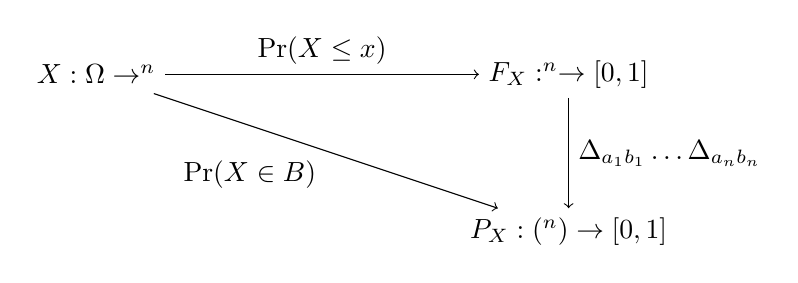
\begin{tikzpicture}
\node (a) at (0,0) {$X:\Omega\to\R^n$};
\node (b) at (6,0) {$F_X:\R^n\to[0,1]$};
\draw[->] (a) -- node[above] {$\Pr(X\leq x)$} (b);
\node (c) at (6,-2) {$P_X:\scB(\R^n)\to[0,1]$};
\draw[->] (b) -- node[right] {$\Delta_{a_1b_1}\dots\Delta_{a_nb_n}$} (c);
\draw[->] (a) -- node[below left] {$\Pr(X\in B)$} (c);
\end{tikzpicture}
\end{center}

这张图的每一个箭头都可以反过来,但是反过来的这些关系都比较不直观,所以我们不再讨论. 

根据上面的讨论,分布函数的特性决定了随机变量的特性. 根据分布函数的不同性质,我们可以将随机变量分为不同的类型. 下面我们将讨论一些重要的类别. 

\subsection{离散型随机变量}\index{随机变量!离散型~}

我们首先讨论\emph{离散型随机变量}. 离散型随机变量的分布函数$F$称之为\emph{离散型分布}\index{分布!离散型~},它是一个阶梯函数,它的函数值只在有限或者可数个点$x_1,x_2,\dots$上发生跳变,在$x_i$的跳变为$p_i=F(x_i)-F(x_i-)$. 这一分布函数对应的概率测度$\Pr$我们称之为\emph{离散型测度}\index{测度!离散型~},这种测度集中在$x_i$上,即$\Pr(X=x_i)=p_i$. 分布函数形如下图:

\begin{center}
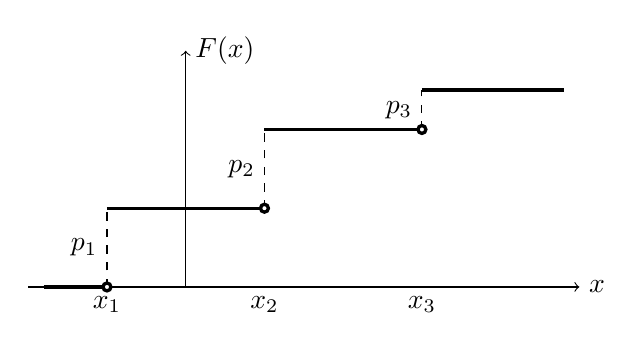
\begin{tikzpicture}
\draw[->] (-2,0) -- (5,0) node[right] {$x$};
\draw[->] (0,0) -- (0,3) node[right] {$F(x)$};
\draw[very thick] (-2+0.2,0) -- (-1,0);
\draw[dashed] (-1,0) -- node[left] {$p_1$} (-1,1);
\draw[very thick] (-1,1) --  (1,1);
\draw[dashed] (1,1) -- node[left] {$p_2$} (1,2);
\draw[very thick] (1,2) -- (3,2);
\draw[dashed] (3,2) -- node[left] {$p_3$} (3,2.5);
\draw[very thick] (3,2.5) -- (5-0.2,2.5);
\draw[fill=white, very thick] (-1,0) circle [radius=0.05];
\draw[fill=white, very thick] (1,1) circle [radius=0.05];
\draw[fill=white, very thick] (3,2) circle [radius=0.05];
\draw (-1,0) node[below] {$x_1$};
\draw (1,0) node[below] {$x_2$};
\draw (3,0) node[below] {$x_3$};
\end{tikzpicture}
\end{center}

离散型分布可以由分布列给出,分布列是一个序列$p_1,p_2,\dots$,其中$p_i=\Pr(X=x_i)$,且$\sum_{i=1}^\infty p_i=1$.

\Cref{tab:discrete-distribution} 列举了一些本书中用到的离散型分布,他们都是整数取值,所以我们记$p_i=\Pr(X=i)$.

\begin{table}[htbp]
\centering
\begin{tabular}{cccc}
\toprule
名称 & 符号 & 分布列 & 参数 \\
\midrule
离散均匀\index{分布!离散均匀~} & $\U[n]$ &$p_i=1/n$,$i=1,\dots,n$ & $n\in\N$ \\
Bernoulli\index{分布!Bernoulli~} & $B(1,p)$ & $p_1=p$,$p_0=1-p$ & $p\in[0,1]$ \\
对称Bernoulli\index{分布!对称Bernoulli~} & — &$p_1=p_{-1}=1/2$ & — \\
二项\index{分布!二项~} &$B(n,p)$ &$p_k=\binom{n}{k}p^k(1-p)^{n-k}$ & $n\in\N$,$p\in[0,1]$ \\
\bottomrule
\end{tabular}
\caption{本书中用到的离散型分布}
\label{tab:discrete-distribution}
\end{table}

\subsection{连续型随机变量}\index{随机变量!连续型~}\label{subsec:continuous-random-variable}

我们再来讨论\emph{连续型随机变量},连续型随机变量的分布函数$F$称为\emph{连续型分布}\index{分布!连续型~},对应的概率测度$\Pr$称之为\emph{绝对连续测度}\index{测度!绝对连续~}. 从名字上就可以看出,测度才是定义连续型随机变量的关键. 我们给出绝对连续测度的定义. 

\begin{definition}[绝对连续测度]\index{测度!绝对连续~}
$\R$上的测度$\Pr$称为\textbf{绝对连续测度},如果对任意$\epsilon>0$,存在$\delta>0$使得任意$A\in\scB(\R)$满足$\lambda(A)<\delta$,都有$\Pr(A)<\epsilon$.
\end{definition}

直观上说,绝对连续测度的意思是当体积$\lambda(\cdot)$发生微小变化的时候(变化量为$\lambda(A)$),测度$\Pr(\cdot)$也只发生微小的变化(变化量为$\Pr(A)$),这和通常函数连续的定义并没有太大的区别. 

那么,绝对连续测度对应的是连续分布函数吗?并非如此!不过,绝对连续测度对应的分布函数有相当漂亮的一种刻画方式:

\begin{theorem}[微积分基本定理]\label{thm:lebesgue-differentiation-theorem}
设$F:\R\to\R$是绝对连续测度对应的分布函数,那么
\[\lambda(\{x\in\R:F'(x)\text{ 不存在}\})=0.\]
定义函数:
\[f(x)=\begin{cases}
    F'(x),&F'(x)\text{ 存在},\\
    0,&\text{其他}.
\end{cases}\]
则$f$是一个非负可积函数,且对任意的$a<b$,都有
\begin{equation}
    F(b)-F(a) = \int_a^b f(x)\d x.\label{eq:Newton-Leibniz}
\end{equation}
\end{theorem}
此处的积分可以理解为Riemann积分或者后面\Cref{sec:expectation} 中的Lebesgue积分. 

\Cref{thm:lebesgue-differentiation-theorem} 意味着,绝对连续测度对应的分布函数几乎处处可以求导,并且所得到的导函数积分回去还是原来的分布函数,也就是微积分基本定理成立. 这样的函数我们称之为\emph{绝对连续函数}\index{绝对连续函数}.

那么,这个$f$应该如何理解呢?先不管\Cref{thm:lebesgue-differentiation-theorem},回到绝对连续测度,仿照导数的定义,考虑极限
\[\frac{\d\Pr}{\d\lambda}(x)=\lim_{\lambda(A)\to 0,x\in A}\frac{\Pr(A)}{\lambda(A)},\]
也就是点$x$附近$\Pr(\cdot)$的微小变化相对于$\lambda(\cdot)$的微小变化.

那么,给定一个集合$A$,要如何求$\Pr(A)$?按照微积分的朴素直观,我们应该将$\Pr$微小的变化转变为$\lambda$微小的变化,也就是积分:
\[\Pr(A)=\int_{x\in A}\frac{\d\Pr}{\d\lambda}(x)\d\lambda(x).\]
我们可以把\eqref{eq:Newton-Leibniz} 改写成如上的形式:
\[\Pr((a,b])=\int_{x\in (a,b]}f(x)\d x.\]
在一维的情况下,$x$的微小变化就是$\lambda(x)$的微小变化,所以$\d x=\d\lambda(x)$. 综合这两点,我们容易相信,
\[f(x)=\frac{\d\Pr}{\d\lambda}(x)\iff \d\Pr=f(x)\d\lambda.\]

所以,$f$应该理解为“密度”. 打个比方,$\lambda$是物体的体积,$\Pr$是物体的质量,那么$f$就是这个物体每个很小的部分上的体积质量除以体积,也就是密度. 所以,我们将$f$称之为\textbf{概率密度函数}\index{概率密度函数},或者简称\textbf{密度}. 通常,$X$的密度记作$p_X$. 

那么,概率测度和密度的区别是什么呢?对于刚接触概率论的人来说,似乎很难理解他们之间的区别. 比如说,有时候会写$p(X=x)$甚至$\Pr(X=x)$来表示密度在$x$处的值$p(x)$,又或者,用$\int\Pr(X=x)\d x$来表示对密度的积分. 这些当然都是不对的,我们下面慢慢论述. 

首先,根据\Cref{thm:lebesgue-differentiation-theorem},$F$是连续函数,所以根据\Cref{ex:distribution-prob},$\Pr(X=x)=F(x)-F(x-)=F(x)-F(x)=0$. 所以$\Pr(X=x)$根本就是零,它和密度函数没有任何关系,所以上面这些写法都是错的. 

那么,要怎么理解密度$p(\cdot)$和概率测度$\Pr(\cdot)$的区别呢?当然,从定义的角度他们就完全不同:一个是从实数到实数的映射,一个是从实数的集合到实数的映射. 但是这样的区别对于初学者来说并不直观. 最直观的区别就在于密度这一词:虽然铅很重(密度大),但是几亿倍于铅体积的棉花却应该比铅重. 所以,密度是微观的,刻画很小部分集合的概率值,也就是$\d\Pr=p_X\d \lambda$;而概率刻画的是宏观的,计算任何一个集合的概率,也就是$\Pr(X\in A)$.

\begin{remark}
    上面的记号$\d\Pr/\d\lambda$并不是随意写出来的,我们叫它导数也不是随意的. 在测度论中,\Cref{thm:lebesgue-differentiation-theorem} 可以被推广为\textbf{Radon-Nikodym定理}\index{Radon-Nikodym定理},这一定理直接保证了形如$\d\Pr/\d\lambda$的函数的存在性,这一函数被称之为\textbf{Radon-Nikodym导数}\index{Radon-Nikodym导数}. 
\end{remark}

利用密度,我们可以很容易计算概率:
\begin{theorem}\label{thm:continuous-prob}
设$X$是一个连续型随机变量,$f$是它的密度函数,则对任意的$B\in\scB(\R)$,都有
\[\Pr(X\in B)=\int_{x\in B}f(x)\d x.\]
\end{theorem}

在\Cref{tab:continuous-distribution} 中,我们给出本书中用到的一些连续型分布的密度函数. 

\begin{table}[htbp]
\centering
\begin{tabular}{cccc}
\toprule
名称 & 符号 & 密度函数 & 参数 \\
\midrule
连续均匀\index{分布!连续均匀~} & $\U(a,b)$ &$p(x)=\frac{1}{b-a}$,$x\in[a,b]$ & $a<b$ \\
指数\index{分布!指数~} & $\Exp(\lambda)$ & $p(x)=\lambda \e^{-\lambda x}$,$x\geq 0$ & $\lambda>0$ \\
双指数\index{分布!双指数~} & $\DExp(\lambda)$ & $p(x)=\frac{\lambda}{2}\e^{-\lambda|x|}$,$x\in\R$ & $\lambda>0$ \\
Laplace\index{分布!Laplace~} & $\Lap(\mu,\lambda)$ & $p(x)=\frac{\lambda}{2}\e^{-\lambda|x-\mu|}$,$x\in\R$ & $\mu\in\R$,$\lambda>0$ \\
正态(Gauss)\index{分布!正态~}\index{分布!Gauss~} & $\Nor(\mu,\sigma^2)$ & $p(x)=\frac{1}{\sqrt{2\pi}\sigma}\e^{-\frac{(x-\mu)^2}{2\sigma^2}}$,$x\in\R$ & $\mu\in\R$,$\sigma>0$ \\
\bottomrule
\end{tabular}
\caption{本书中用到的连续型分布}
\label{tab:continuous-distribution}
\end{table}

\begin{remark}
从\Cref{thm:lebesgue-differentiation-theorem} 来看,密度函数的定义似乎是唯一的,但是从积分的角度,如果密度函数在几个点上的值发生了变化,并不影响整个积分的值,从而也不影响求概率. 比如均匀分布$\U(a,b)$,端点$a,b$的值到底是$0$还是$1/(b-a)$并不重要,取任何一个值都是可以的.     
\end{remark}

\begin{remark}
密度函数通常是需要分段写出的,比如,$U(a,b)$的密度函数,严格来说应该写为
\[p(x)=\begin{cases}
    0,&x<a,\\
    \frac{1}{b-a},&x\in[a,b],\\
    0,&x>b.
\end{cases}\]
为了简化记号,我们可以用\textbf{示性函数}\index{示性函数}来表示这一分类. 设$A\subseteq\R$,定义函数
\[I_A(x)=\begin{cases}
    1,&x\in A,\\
    0,&x\notin A.
\end{cases}\]
则$U(a,b)$的密度函数可以写为
\[p(x)=\frac{1}{b-a}I_{[a,b]}(x).\]

更一般地,示性函数中的字母$A$可以是任意一个事件,而关于事件的那些记号都可以在$A$这里写出. 示性函数在概率论中有着核心的作用,我们在后面将会经常用到示性函数. 
\end{remark}

\subsection{随机向量,条件分布,独立性}\label{subsec:random-vector}

我们前面已经说过,随机向量就是$\Omega\to\R^n$的映射. $n$维的随机向量可以看成$n$个随机变量的组合,可以写作$X=(X_1,\dots,X_n)^\t$. 通常,我们将$X$的分布函数称为$X_1,\dots,X_n$的\emph{联合分布}\index{分布!联合~},将$X_i$的分布函数称为$X$的\emph{边缘分布}\index{分布!边缘~}.

关于随机变量的分类可以完全平行移植到随机向量上. 下面我们分别讨论. 

离散型随机向量指的是它对应的概率测度集中在有限或可数个点上. 这样的分布依然可以用分布列给出:$\Pr(X_1=x_1,\dots,X_n=x_n)=p_{x_1,\dots,x_n}$,其中$x_i$取遍所有可能的值. 

本书中使用的离散型随机向量只有多项分布\index{分布!多项~},符号为$PN(n,p_1,\dots,p_k)$,分布列为
\[\Pr(X_1=i_1,\dots,X_n=i_n)=\frac{n!}{i_1!\cdots i_k!}p_1^{i_1}\cdots p_k^{i_k},\]
其中$n\in\N$,$p_i\geq 0$,$\sum_{i=1}^k p_i=1$. 

连续型随机向量指的是它对应的概率测度是绝对连续的. 连续型随机向量的分布函数依然由绝对连续函数刻画:

\begin{theorem}\label{thm:continuous-vector}
设$F:\R^n\to\R$是绝对连续测度对应的分布函数,那么存在一个非负可积函数$f:\R^n\to\R$,使得对任意的$(x_1,\dots,x_n)\in\R^n$,都有
\[F(x_1,\dots,x_n)=\int_{-\infty}^{x_1}\cdots\int_{-\infty}^{x_n}f(y_1,\dots,y_n)\d y_1\cdots\d y_n.\]
\end{theorem}

此时,$f$称为$X$的\textbf{概率密度函数}\index{概率密度函数},或者简称\textbf{密度}. 通常,$X$的密度记作$p_X$.

类似随机变量的讨论,密度函数依然可以被写做导数的形式. 假设$\Pr$是绝对连续测度,它对应的密度是$p$,那么
\[\frac{\d\Pr}{\d\lambda}(x)=p(x)\iff \d\Pr=p(x)\d\lambda.\]

这里,我们需要再给出一些$\d\lambda$和$\d x$关系的讨论. $\d\lambda$应该理解为Lebesgue测度的微小变化,然而我们并不假定这一变化是如何产生的. $\d x$理解为$x$的微小变化. $x$的微小变化自然就产生了$\lambda$的微小变化,即$\lambda(\d x)$. 所以,在$x$处,$\d\lambda$和$\d x$之间的关系应该是$\d\lambda=\lambda(\d x)$,于是$\d\lambda$应该理解为$\d x$形成的长方体的体积. 

同样,密度给出了概率计算的一个重要工具:
\begin{theorem}\label{thm:continuous-prob-vec}
    设$X$是一个$n$维连续型随机向量,$f$是它的密度函数,则对任意的$B\in\scB(\R^n)$,都有
    \[\Pr(X\in B)=\int_{x\in B}f(x)\d x.\]
\end{theorem}

利用联合密度,可以计算边缘密度:
\begin{theorem}\label{thm:continuous-marginal}
    设$X=(X_1,\dots,X_n)$是一个$n$维连续型随机向量,,则对任意的$1\leq i\leq n$,都有
    \[p_{X_i}(x_i)=\int_{(x_1,\dots,x_{i-1},x_{i+1},\dots,x_n)\in\R^{n-1}}p_X(x_1,\dots,x_n)\d x_1\cdots\d x_{i-1}\d x_{i+1}\cdots\d x_n.\]
\end{theorem}

这一命题当然也可以自然推广到求随机向量的边缘密度,例如利用$X=(X_1,X_2,X_3)$的联合密度计算$(X_1,X_2)$的边缘密度:
\[
    p_{X_1,X_2}(x_1,x_2) = \int_{x_3\in\R}p_X(x_1,x_2,x_3)\d x_3.
\]

连续型随机变量的一个重要的例子是多元正态分布,或者(非退化)Gauss向量\index{分布!多元正态~}\index{Gauss向量}. 它的密度函数为
\[p(x)=\frac{1}{(2\pi)^{n/2}\sqrt{\det\Sigma}}\e^{-\frac{1}{2}(x-\mu)^\t\Sigma^{-1}(x-\mu)},\]
其中$\mu\in\R^n$,$\Sigma$是一个$n\times n$的正定矩阵. 这一分布的符号是$\Nor(\mu,\Sigma)$. 

关于Gauss向量的性质,我们将在\Cref{sec:multivariate-normal} 中讨论. 

接下来,我们讨论条件分布. 

对于离散型随机向量$X=(X_1,X_2)$,它的分布完全由分布列给出. 我们可以定义$X_1$在给定$X_2$的条件下的分布列:
\[\Pr(X_1=x_1|X_2=x_2)=\frac{\Pr(X_1=x_1,X_2=x_2)}{\Pr(X_2=x_2)}.\]
由此给出了随机变量$X_1$在给定$X_2$的条件下的\emph{条件分布列},继而给出了\emph{条件分布}\index{分布!条件~}. 这一定义也可以推广到$X_i$是随机向量的情况. 

然而,对于一般的随机向量,特别是连续型随机向量,这一定义是行不通的. 比如,如果$X=(X_1,X_2)$是连续型随机向量,那么 $\Pr(X_2=x_2)=\Pr(X_1=x_1,X_2=x_2)=0$,所以条件概率的分子和分布概率都是零,这样的定义是没有意义的. 

转换思路,去尝试定义所谓的\emph{条件分布函数}:$\Pr(X_1\leq x_1|X_2=x_2)$. 考虑$\Pr(X_1\leq x_1|x_2< X_2\leq x_2+\epsilon)$,再令$\epsilon\downarrow 0$,我们有如下计算:
\begin{align*}
    &\lim_{\epsilon\downarrow 0}\Pr(X_1\leq x_1|x_2< X_2\leq x_2+\epsilon) \\
    =&\lim_{\epsilon\downarrow 0}\frac{\Pr(X_1\leq x_1,X_2\leq x_2+\epsilon)-\Pr(X_1\leq x_1,X_2\leq x_2)}{\Pr(x_2< X_2\leq x_2+\epsilon)}\\
    =&\lim_{\epsilon\downarrow 0}\frac{F_X(x_1,x_2+\epsilon)-F_X(x_1,x_2)}{F_{X_2}(x_2+\epsilon)-F_{X_2}(x_2)}.
\end{align*}

如果上面的极限存在,我们就定义它是$X_1$在给定$X_2$的条件下的\emph{条件分布}\index{分布!条件~}. 

如果$X$是连续性随机变量,我们还可以继续算下去:
\begin{align*}
    &\lim_{\epsilon\downarrow 0}\frac{F_X(x_1,x_2+\epsilon)-F_X(x_1,x_2)}{F_{X_2}(x_2+\epsilon)-F_{X_2}(x_2)}\\
    =&\frac{\partial F_X(x_1,x_2)}{\partial x_2}\frac{1}{p_{X_2}(x_2)}\\
    =&\int_{-\infty}^{x_1}\frac{\partial^2 F_X(y,x_2)}{\partial x_2\partial y}\frac{1}{p_{X_2}(x_2)}\d y\\
    =&\int_{-\infty}^{x_1}\frac{p_{X_1,X_2}(y,x_2)}{p_{X_2}(x_2)}\d y.
\end{align*}

对照\Cref{thm:lebesgue-differentiation-theorem},我们知道$p_{X_1,X_2}/p_{X_2}$具有密度函数的形式,所以连续性随机向量所定义的条件分布也是连续型分布,密度函数被$p_{X_1,X_2}/p_{X_2}$通常记作$p_{X_1|X_2}$,称为$X_1$在给定$X_2$的条件下的\emph{条件密度}. 

以上讨论也可以自然推广到$X_i$是随机向量的情况,我们就不给出了. 

最后,我们讨论随机向量之间的独立性. 随机向量之间的独立性完全由事件的独立性刻画,所以我们有如下定义:

\begin{definition}[随机向量的独立性]\index{独立性}
设$X_1,\dots,X_n$是$n$个随机向量,第$i$个的维数是$n_i$. 如果对任意的$1\leq i_1,\dots,i_k\leq n$,以及任意的$B_{i_1}\in\scB(\R^{n_{i_1}}),\dots,B_{i_k}\in\scB(\R^{n_{i_k}})$,都有
\[\Pr(X_{i_1}\in B_{i_1},\dots,X_{i_k}\in B_{i_k})=\Pr(X_{i_1}\in B_{i_1})\cdots\Pr(X_{i_k}\in B_{i_k}),\]
则称$X_1,\dots,X_n$是\textbf{独立的}. 

特别地,如果$X_1,\dots,X_n$是一维的,那么这定义了随机变量之间的独立性. 
\end{definition}

这一定义中包含了无穷多个需要验证的等式,利用分布函数,我们可以将独立性的验证转化为一个等式的验证:

\begin{theorem}\label{thm:independence}
设$X_1,\dots,X_n$是$n$个随机向量,第$i$个的维数是$n_i$,$F_i$是$X_i$的分布函数,$F$是$(X_1,\dots,X_n)$的联合分布函数. $X_1,\dots,X_n$独立的充分必要条件是
\[F(x_1,\dots,x_n)=F_1(x_1)\cdots F_n(x_n),\]
其中$x_i\in\R^{n_i}$.
\end{theorem}

对于离散型随机向量,它的分布函数完全由分布列决定,所以\Cref{thm:independence} 等价于如下命题:

\begin{proposition}\label{prop:independence-discrete}
设$X_1,\dots,X_n$是$n$个离散型随机向量,第$i$个的维数是$n_i$,$p_i$是$X_i$的分布列,$p$是$(X_1,\dots,X_n)$的联合分布列. $X_1,\dots,X_n$独立的充分必要条件是
\[p(x_1,\dots,x_n)=p_1(x_1)\cdots p_n(x_n),\]
其中$x_i\in\R^{n_i}$.
\end{proposition}

对于连续型随机向量,它的分布函数完全由密度决定,所以\Cref{thm:independence} 等价于如下命题:

\begin{proposition}\label{prop:independence-continuous}
设$X_1,\dots,X_n$是$n$个连续型随机向量,第$i$个的维数是$n_i$,$p_i$是$X_i$的密度函数. 假设他们的联合分布具有密度函数$p$. $X_1,\dots,X_n$独立的充分必要条件是
\[p(x_1,\dots,x_n)=p_1(x_1)\cdots p_n(x_n),\]
其中$x_i\in\R^{n_i}$.
\end{proposition}

上面两个命题都有更简单的形式:

\begin{corollary}\label{cor:independence-continuous}
设$X_1,\dots,X_n$是$n$个连续型(离散型)随机向量,第$i$个的维数是$n_i$,假设他们的联合分布具有密度函数(分布列)$p$. $X_1,\dots,X_n$独立的充分必要条件存在函数$f_1,\dots,f_n$使得
\[p(x_1,\dots,x_n)=f_1(x_1)\cdots f_n(x_n),\]
其中$x_i\in\R^{n_i}$.
\end{corollary}

利用这一命题,判断独立性的时候,我们只要尝试将联合密度(分布列)分解成若干个函数的乘积即可. 

对于连续型随机向量,这一判据特别要注意密度函数的分段情况. 比如,考虑$X=(X_1,X_2)$,其密度函数为
\[p(x_1,x_2)=\begin{cases}
    8x_1x_2,& 0\leq x_1\leq x_2,0\leq x_2\leq 1,\\
    0,&\text{其他}.
\end{cases}\]
如果忽略了$x_i$的取值范围,我们很容易以为$p(x_1,x_2)$可以写成$f(x_1)f(x_2)$,所以他们独立. 然而事实并不是这样的!计算$X_1$的边缘密度:
\[p_1(x_1)=\int_{x_2\in\R}p(x_1,x_2)\d x_2=\begin{cases}
    4x_1(1-x_1^2),&0\leq x_1\leq 1,\\
    0,&\text{其他}.
\end{cases}\]
再计算$X_2$的边缘密度:
\[p_2(x_2)=\int_{x_1\in\R}p(x_1,x_2)\d x_1=\begin{cases}
    4x_2^3,&0\leq x_2\leq 1,\\
    0,&\text{其他}.
\end{cases}\]
显然,$p_1(x_1)\cdot p_2(x_2)\neq p(x_1,x_2)$,所以$X_1,X_2$不独立. 

如果使用示性函数\index{示性函数}来书写密度函数,这一问题更不容易被忽视,在上面的例子中,$p(x_1,x_2)=8x_1x_2I_{0\leq x_1\leq x_2\leq 1}(x_1,x_2)$,示性函数显然是拆不成分别只关于$x_1$和$x_2$的函数乘积的. 

自然,利用条件分布,我们可以给出独立的另一种刻画:

\begin{proposition}\label{prop:independence-conditional}
设$X_1,X_2$是两个随机变量,他们的联合分布是离散型或连续型的. $X_1,X_2$独立的充分必要条件是对任意的$x_1,x_2$,都有
\[\Pr(X_1\leq x_1|X_2=x_2)=\Pr(X_1\leq x_1).\]
如果$X_1,X_2$是离散型的,那么这一条件可以改写为
\[\Pr(X_1=x_1|X_2=x_2)=\Pr(X_1=x_1).\]
如果$X_1,X_2$是连续型的,那么这一条件可以改写为
\[p_{X_1|X_2}(x_1|x_2)=p_{X_1}(x_1).\]
\end{proposition}

注意,上述判据并不需要真的把等式右边的量算出来,我们只需要判断刻画条件分布的量(条件分布函数、条件分布列或条件密度)中,是不是只出现了$x_1$而没有出现$x_2$. 

\subsection{随机变量(向量)的函数}\label{subsec:random-function}

我们前面说过,如果$X$是随机向量,$g$是一个Borel函数,那么$g(X)=g\circ X$也是一个随机向量. 这里,记号$g\circ X$将$X$看成一个映射,于是得到的是一个复合函数;而记号$g(X)$则更直观,它表示把$X$看成一个数学对象(随机向量),然后对它进行函数运算,得到另一个同类型的数学对象(随机向量). 我们将始终采取后者的记号,但请务必注意,符号$g(X)$中的$X$绝对不应该理解为一个数,而应该理解为一个随机向量. 

随机变量的函数最直接的问题就是,它的分布是什么?我们只关注离散型和连续型随机向量的情况.

对于离散型随机向量,它的分布完全由分布列决定,很容易得到如下命题:

\begin{theorem}\label{thm:discrete-function}
设$X$是一个离散型随机向量,$g$是一个函数,那么$Y=g(X)$也是一个离散型随机向量,它的分布列为
\[\Pr(Y=y)=\sum_{x\in g^{-1}(y)}\Pr(X=x).\]
\end{theorem}

对于连续型随机向量,它的分布完全由密度决定. 我们现在来推导连续型随机向量的函数的密度. 

设$X$是一个$n$维连续型随机向量,$g\in C^1(\R^n,\R^n)$,即$\R^n\to\R^n$的连续可微函数. 为了简便起见,我们假设$g$是单射,并且反函数也连续可微. 设$Y=g(X)$,可以证明,$Y$是一个连续型随机向量. 

我们现在来计算$Y$的密度. 考虑$Y$取值的一个微小的区域$\d y$,$\d P_Y=p_Y\lambda(\d y)$是$Y$在$\d y$上的概率,同样区域的概率也可以用$X$去计算:
\[\d P_X=p_X\lambda(\d x),\quad Y\in\d y\iff X\in\d x,\]
当然,这里$\d y$和$\d x$由函数$g$联系在一起,因为$Y=g(X)$,所以$\d y/\d x=g'(X)$,注意,这相当于微元$\d y$和微元$\d x$的有向体积的比. 最后,根据概率相等,可以写出如下的等式:
\begin{equation}
    \d P_Y=\d P_X\iff p_Y\lambda(\d y)=p_X\lambda(\d x).\label{eq:eq-prob}
\end{equation}
考虑到密度是计算体积而非有向体积,根据Jacobi行列式\index{Jacobi行列式}的几何意义(见\Cref{subsec:partial-derivative}),
\[p_Y(y)=\left|\frac{\d x}{\d y}\right|p_X(x)=\left|\frac{\d y}{\d x}\right|^{-1}p_X(x)=|\det g'(x)|^{-1}p_X(x).\]
这就得到了$Y$的密度函数. 

如果$g$不是单射,那么上面的 \eqref{eq:eq-prob} 需要考虑$g$每一个单射的局部. 例如,如果$g(x)=x^2$,那么$g$在$(0,+\infty)$上和$(-\infty,0)$上都是单射,一个$y$对应了两个$x$. 在这种情况下,每一个$y$所对应的$x$都贡献了概率,所以 \eqref{eq:eq-prob} 需要写成
\begin{equation}
    \d P_Y=\sum_{g(x)=y}\d P_X(x)\iff p_Y\lambda(\d y)=\sum_{g(x)=y}p_X(x)\lambda(\d x)(x).\label{eq:eq-prob-2}
\end{equation}
总结以上讨论,我们得到连续型随机向量的函数的密度的计算公式:

\begin{theorem}\label{thm:continuous-function}
设$X$是一个连续型随机向量,$g\in C(\R^n,\R^n)$,即$\R^n\to\R^n$的连续函数,假设$\lambda(\{x\in\R^n:\det g'(x)\neq 0\})=0$,则$Y=g(X)$也是一个连续型随机向量,它的密度函数为
\[p_Y(y)=\begin{cases}
    \sum_{g(x)=y}|\det g'(g^{-1}(y))|^{-1}p_X(g^{-1}(y)),&\det g'(g^{-1}(y))\neq 0,\\
    0,&\text{其他}.
\end{cases}\]
其中求和号中$g^{-1}(y)$是根据相应的$x$,用反函数定理(\Cref{thm:inverse-function})\index{反函数定理}求出局部反函数. 
\end{theorem}

这一定理的表述比较宽泛,我们可以给一个具体的例子来理解. 

\begin{example}
设$X$是一个连续型随机变量,$g(x)=x^2$,我们来计算$Y=X^2=g(X)$的密度. 直接计算\Cref{thm:continuous-function} 中的公式,我们有
\begin{align*}
    &\sum_{g(x)=y}|\det g'(g^{-1}(y))|^{-1}p_X(g^{-1}(y))\\
    =&\sum_{x^2=y}\frac{1}{2|x|}p_X(x)\\
    =&\frac{1}{2\sqrt{y}}p_X(\sqrt{y})+\frac{1}{2\sqrt{y}}p_X(-\sqrt{y}).
\end{align*}
这就给出了$Y$的密度. 
\end{example}

一般来说,\Cref{thm:continuous-function} 中的公式并不好记,最实用的还是根据$X$和$Y$在算相同的概率这一事实直接写出 \eqref{eq:eq-prob-2},然后根据具体的$g$来计算. 比如上面的例子,我们可以直接写出
\[p_Y\lambda(\d y)=p_X(\sqrt{y})\lambda(\d x)(\sqrt{y})+p_X(-\sqrt{y})\lambda(\d x)(-\sqrt{y}).\]
两边除以$\lambda(\d y)$,再利用$\d y/\d x=1/(2x)$,就得到了$Y$的密度. 

最后,如果映射$g$并不是保持维度的,例如$g:\R^n\to\R^m$,但$m<n$\footnote{如果$m>n$,那么$g(X)$一定不会是连续型随机变量,因为它的每个维之间一定会产生相互的关联,所以我们不讨论这种情况. },那么我们可以将$g$补全到$n$维映射,也就是说,我们可以定义一个新的函数$G:\R^n\to\R^n$满足
\[G(x_1,\dots,x_n)=(g_1(x_1,\dots,x_n),\dots,g_m(x_1,\dots,x_n),x_{m+1},\dots,x_n)^\t.\]
然后,利用这一函数计算出$g(X)$和$(X_{m+1},\dots,X_n)$的联合概率密度,再求出$g(X)$的边缘密度. 

我们看一个简单的例子. 

\begin{example}[卷积]
设$X,Y$是随机变量,我们来计算$Z=X+Y$的密度. 我们可以将$Z$看成是$g(X,Y)=(X+Y,Y)$的第一个维度. 映射$(x,y)\mapsto(x+y,y)$显然是双射,所以 \eqref{eq:eq-prob-2} 退化为 \eqref{eq:eq-prob},我们有
\[p_{Z,Y}(z,y)=\left|\frac{\partial(z,y)}{\partial(x,y)}\right|^{-1}p_{X,Y}(x,y)=p_{X,Y}(z-y,y).\]
于是,$Z$的边缘密度为
\[p_Z(z)=\int_{y\in\R}p_{X,Y}(z-y,y)\d y.\]
这被称为$X$和$Y$的\textbf{卷积}\index{卷积}. 
\end{example}

最后,对随机向量作用函数是不会影响独立性的:

\begin{proposition}\label{prop:independence-function}
设$X_1,\dots,X_n$是$n$个随机向量,第$i$个的维数是$n_i$,$g_i$是$\R^{n_i}\to\R^{m_i}$的Borel函数,$Y_i=g_i(X_i)$,如果$X_1,\dots,X_n$相互独立,那么$Y_1,\dots,Y_n$也相互独立. 
\end{proposition}

\section{随机变量的数字特征,条件数学期望}\label{sec:expectation}

分布函数或者随机变量依然是一个映射,研究起来还是会比较复杂. 我们希望能够用一些数字来刻画随机变量的特征,这样可以进一步简化问题. 在这一节中,我们将介绍随机变量的数字特征,以及条件数学期望. 

\subsection{数学期望,Lebesgue积分}

数学期望在数学上是很直观的,我们可以从一个赌博的例子入手来找一些感觉. 

\begin{example}
在一个地下赌场,有赌徒甲乙两人. 这是一个公平的赌局,每局甲乙获胜概率都是$1/2$,每局各出赌注$50$块. 谁先赢到三局,就可以赢得全部的赌注. 赌博进行了三轮,甲赢了两局,乙赢了一局. 这时,突然有消息说警察马上就要来查封赌场,甲乙于是决定将目前的所有赌资进行分割. 他们应该如何分割呢?

再赌两盘就会决出胜负,赌博一共会有三种可能:
\begin{enumerate}
    \item 第四盘甲赢,于是甲赢的所有赌注,这样的概率是$1/2$;
    \item 第四盘乙赢,第五盘甲赢,于是甲赢的所有赌注,这样的概率是$(1/2)\times(1/2)=1/4$;
    \item 乙连赢两盘,于是乙赢的所有赌注,这样的概率是$(1/2)\times(1/2)=1/4$. 
\end{enumerate}
现在的赌资是$100\times 3=600$块,甲有$1/2+1/4=3/4$的概率会拿到全部,乙有$1/4$的概率会拿到全部. 于是,按照概率去平分的话,甲应该拿走$450$块,乙应该拿走$150$块. 
\end{example}

这个例子说明了期望的一种理解方式:在面对随机性的时候,我们按照概率的权重分配. 比如,上面的例子中,设$X$是甲赢的赌注,那么$X$的分布列为$\Pr(X=0)=1/4$,$\Pr(X=600)=3/4$,所以$\E[X]=0\times 1/4+600\times 3/4=450$.

以上的例子给了我们定义随机变量期望的基础:定义\emph{示性函数}\index{示性函数}的数学期望. 设$A$是一个事件,那么$I_A$是一个随机变量:
\[I_A(\omega)=\begin{cases}
    1,&\omega\in A,\\
    0,&\omega\notin A.
\end{cases}\]
我们称之为事件$A$的\emph{示性函数}. 示性函数的分布列是
\[\Pr(I_A=1)=\Pr(A),\quad \Pr(I_A=0)=\Pr(A^c)=1-\Pr(A).\]
所以,示性函数的数学期望,按照上面的逻辑,应该是
\[\E[I_A]=1\times\Pr(A)+0\times\Pr(A^c)=\Pr(A).\]

示性函数建立了概率和数学期望的联系. 下面,我们来定义一般随机变量的数学期望,这一定义的过程反映了一种数学的思想:用简单东西的极限去研究复杂的东西. 

第一步,定义\emph{示性函数}的数学期望\footnote{从逻辑上说,示性函数的数学期望是被定义出来的,而不是被算出来的,因为此时我们还完全没有定义什么是数学期望. }. $\E[I_A]=\Pr(A)$.

第二步,定义\emph{简单随机变量}的数学期望. 简单随机变量是形如$X=\sum_{k=1}^n x_kI_{A_k}$的随机变量,其中$x_k\in\R$,$A_k$是事件. 定义
\[\E[X]=\sum_{k=1}^n x_k\Pr(A_k).\]
这一定义与第一步是相容的:因为$I_A=1\cdot I_{A}$,所以$\E[I_A]=1\cdot\Pr(A)=\Pr(A)$. 

第三步,定义\emph{非负随机变量}的数学期望. 非负随机变量是指$X(\omega)\geq 0$对任意$\omega$成立的随机变量$X$. 考虑一列简单随机变量$\{X_n\}_{n=1}^\infty$,它满足对于每一个$\omega\in\Omega$都有当$n\to\infty$时$X_n(\omega)\uparrow X(\omega)$. 容易验证,$\E[X_n]$也是单调递增的,所以根据\Cref{prop:monotone-bounded},$\E[X_n]$有有限的极限或者趋于正无穷,我们都记为$\lim_{n\to\infty} \E[X_n]$.

\begin{definition}[数学期望(Lebesgue积分),非负情形]\index{数学期望}\index{Lebesgue积分}
称
\[\E[X]=\lim_{n\to\infty}\E[X_n]\]
为随机变量$X$的\textbf{数学期望}或\textbf{Lebesgue积分}. 
\end{definition}

可以证明,这一定义不依赖于$\{X_n\}_{n=1}^\infty$的选取,因而是良定义的. 此外,容易看出,这一定义与第二步是相容的,所以第三步扩展了第二步的定义. 

第四步,定义\emph{一般随机变量}的数学期望. 考虑随机变量$X$,定义$X^+=\max\{X,0\}$,$X^-=-\min\{X,0\}$,也就是$X$的正数部分和负数部分,那么$X=X^+-X^-$. 我们有如下定义:

\begin{definition}[数学期望(Lebesgue积分),一般情形]\index{数学期望}\index{Lebesgue积分}
称随机变量$X$的数学期望\textbf{存在},如果$\E[X^+]$和$\E[X^-]$至少有一个有限. 此时,定义
\[\E[X]=\E[X^+]-\E[X^-]\]
为随机变量$X$的\textbf{数学期望}或\textbf{Lebesgue积分}. 

如果$\E[X^+]$和$\E[X^-]$都是有限的,那么称$X$有\textbf{有限期望}或\textbf{可积的}. 
\end{definition}

当我们强调积分的时候,$\E[X]$也会写为
\[E[X]=\int_\Omega X\d\Pr.\]

以上定义适用于任何一种概率空间和概率测度. 容易看出来,这一定义也适用于$\R^n$上的Lebesgue测度,我们唯一需要改变的就是示性函数的Lebesgue积分的定义:对任意$A\in\scB(\R^n)$,定义
\[\int_{\R^n} I_A(\omega)\lambda(\d \omega)=\lambda(A).\]
然后对简单函数定义积分,再对非负函数定义积分,最后对一般函数定义积分. 

对于$\R^n$上的Lebesgue积分,我们一般省略$\lambda$\footnote{对于一维的情况,见\Cref{subsec:continuous-random-variable} 的讨论. 在高维空间中,这样的记号其实是相当糟糕的:在微分学中,求导数时,$\d x$被理解为切空间的向量,或者一个微小的位移;求然而在积分学中,$\d x$被理解为所对应平行体的体积. 所以其实$\lambda(\d x)$这一记号虽然复杂,但是含义更准确. },直接写成
\[\int_{\R^n} f(x)\d x.\]
这与我们所熟知的积分符号就完全一致了. 

上面定义随机变量期望的过程中,最难以理解的是第三步,也就是非负随机变量的数学期望. 我们来具体算一下它的表达式. 

设$X$是一个非负随机变量,分布为$F$. 我们来计算$\E[X]$,与其说是计算,不如说重新推导一遍第三步的过程. 首先,我们将$X$取值范围离散化,每$1/n$一段,$X$的值都压到形如$k/n$的点上,这样就转化为了一个离散型随机变量:
\[X_n=\sum_{k=0}^\infty\frac{k}{n}I_{\{k/n\leq X<(k+1)/n\}}.\]
容易看出,$X_n(\omega)\uparrow X(\omega)$对任意$\omega$成立. 于是,我们有
\[\E[X]=\lim_{n\to\infty}\E[X_n].\]
我们来计算$\E[X_n]$,注意到$X_n$是一个简单随机变量,我们有
\begin{align*}
    \E[X_n]=&\sum_{k=0}^\infty\frac{k}{n}\Pr\left(\frac{k}{n}\leq X<\frac{k+1}{n}\right)\\
    =&\sum_{k=0}^\infty\frac{k}{n}\left(F\left(\frac{k+1}{n}\right)-F\left(\frac{k}{n}\right)\right).
\end{align*}
按照极限的想法,当$n\to\infty$时,上式的求和项相当于$x\d F(x)$,这里$\d F$表示$x$微小变化时对应的$F$的微小变化. 所以形式上我们有
\[\E[X]=\int_{x\geq 0} x\d F(x)=\int_\R x\d F(x),\]
这里第二个等式是因为在$x<0$的时候$F$恒等于$0$,因而可以理解为$\d F(x)=0$.

如果$X$不是非负的,那么对$X^+$和$X^-$分别计算数学期望,然后相减,就得到了一般随机变量的数学期望,它依然满足:
\[\E[X]=\int_{\R} x\d F(x).\]
所以,随机变量的数学期望完全取决于它的分布函数. 

对于离散型随机变量来说,$F$只在点$x_1,x_2,\dots$会发生改变,其他地方都是常值,所以我们有
\[\int_{\R} x\d F(x)=\sum_{k=1}^\infty x_k(F(x_k)-F(x_k-))=\sum_{k=1}^\infty x_k\Pr(X=x_k).\]

对于连续型随机变量来说,$\d F=p\d x$,这里$p$是对应的密度. 于是我们有
\[\int_{\R} x\d F(x)=\int_{\R} x p(x)\d x.\]

以上就是概率论中常见的求期望的形式. 

我们再介绍一个非常有用的符号,它允许我们在某个事件$A$上求积分:
\[\int_A X\d\Pr=\int_{\Omega} XI_A\d\Pr=\E[XI_A].\]
相应地,在$\R^n$上,对我们也可以定义
\[\int_A f(x)\lambda(\d x)=\int_{\R^n} f(x)I_A(x)\lambda(\d x).\]


刻画随机变量的数字特征,除了可以用随机变量的期望,还可以用随机变量的函数的期望,我们列举一个重要的概念. 

\begin{definition}[矩,方差,特征函数]\index{矩}\index{方差}\index{特征函数}
设$X$是一个随机变量,我们有如下定义:
\begin{itemize}
    \item $k$是一个正整数,称$\E[X^k]$为$X$的\textbf{$k$阶矩};称$\E[(X-\E[X])^k]$为$X$的\textbf{$k$阶中心矩};
    \item 称$\E[(X-\E[X])^2]$为$X$的\textbf{方差},记为$\var(X)$;
    \item 称$f_X(t)=\E[\exp(i tX)]$为$X$的\textbf{特征函数}. 一般地,如果$X$是$n$维随机向量,那么$f_X:\R^n\to\C$,$f_X(t)=\E[\exp(i\inner{t}{X})]$被称为$X$的\textbf{特征函数}. 
\end{itemize}
\end{definition}
我们将会在后面讨论他们的性质. 

\subsection{数学期望的性质}

我们已经给出了数学期望的定义,下面我们罗列一些数学期望的性质,但都不给出证明. 

\begin{proposition}\label{prop:expectation-property}
\begin{enumerate}
\item 期望的线性性:设$X,Y$是随机变量,$a,b\in\R$,如果$\E[X]$和$\E[Y]$都存在,那么$\E[aX+bY]$存在,且
\[\E[aX+bY]=a\E[X]+b\E[Y].\]
\item 单调性:设$X,Y$是随机变量,如果$X\leq Y$,那么
\[\E[X]\leq \E[Y].\]
\item 绝对值不等式:设$X$是随机变量,那么
\[\E[|X|]\geq |\E[X]|.\]
\item 局部可积性:设$X$是随机变量,并且$\E[X]$存在,那么对任意事件$A$,$\E[XI_A]$也存在;如果$\E[X]$有限,那么$\E[XI_A]$也有限. 
\end{enumerate}
\end{proposition}

接下来,我们讨论随机变量函数的期望的求法. 假设$X$是一个$n$维随机向量,$g:\R^n\to\R$是一个Borel函数,那么$g(X)$也是一个随机变量(\Cref{thm:random-variable}). 计算$\E[g(X)]$有以下两种方式,我们下面分别讨论. 

第一种,利用\Cref{subsec:random-function} 中的方法,我们可以将$g(X)$的分布写出来,然后计算期望. 我们来看一个例子. 

\begin{example}\label{ex:uniform-square}
设$X\sim\U(0,1)$,计算$\E[X^2]$. 直接算出$Y=X^2$的密度函数为
\[p_Y(y)=\begin{cases}
    \frac{1}{2\sqrt{y}},&0\leq y\leq 1,\\
    0,&\text{其他}.
\end{cases}\]
于是,
\[\E[X^2]=\int_{\R} y p_Y(x)\d y=\int_0^1\frac{y}{2\sqrt{y}}\d y=\frac{1}{3}.\]
\end{example}

第二种,我们从定义出发,直接计算$\E[g(X)]$. 我们先考虑最简单的情况,即$g$连续并且$0\leq g\leq C$的情况,这里$C$是一个正常数. 我们还是试图使用第三步,用简单随机变量去逼近$g(X)$. 我们选择离散化$X$,还是一样定义
\[X_n=\sum_{k=0}^\infty\frac{k}{n}I_{\{k/n\leq X<(k+1)/n\}}.\]
可以证明\footnote{注意,这里$g(X_n)$未必单调趋于$g(X)$了,所以这里我们其实跳了一个比较重要的步骤,即不单调趋于的时候极限也可以拿到期望外面. 由于这一步的证明比较技术,而且对本书的讨论不是特别重要,所以这里略去. }
\[\E[g(X)]=\lim_{n\to\infty}\E[g(X_n)].\]
用$X$的分布函数$F$写出来$\E[X_n]$就是
\begin{align*}
    \E[X_n]=\sum_{k=0}^\infty g\left(\frac{k}{n}\right)\left(F\left(\frac{k+1}{n}\right)-F\left(\frac{k}{n}\right)\right).
\end{align*}
取极限,写成积分的形式,我们有:
\[\E[g(X)]=\int_{\R} g(x)\d F(x).\]

利用逼近的思想,我们可以将上述结论推广到$g$是任意的Borel函数的情况,于是我们有:

\begin{theorem}\label{thm:expectation-function}
设$X$是一个$n$维随机向量,每一维都可积,$g:\R^n\to\R$是一个Borel函数,那么$\E[g(X)]$存在,且
\[\E[g(X)]=\int_{\R^n} g(x)\d F_X(x).\]
特别地,如果$X$是一个离散型随机变量,取值为$x_1,x_2,\dots$,那么
\[\E[g(X)]=\sum_{k=1}^\infty g(x_k)\Pr(X=x_k).\]
如果$X$是一个连续型随机变量,密度为$p_X$,那么
\[\E[g(X)]=\int_{\R^n} g(x)p_X(x)\d x.\]
\end{theorem}

\begin{example}
我们重新算一次上面的\Cref{ex:uniform-square},这次我们用\Cref{thm:expectation-function} 来计算. 设$X\sim\U(0,1)$,我们有
\[E[X^2]=\int_0^1 x^2\d x=\frac{1}{3}.\]
\end{example}

从这两个例子就可以看出,以上两种方法,通常来说第二种会更加容易计算一些,因为它只需要做一次积分,而第一种方法还需要算变量替换的Jacobi行列式. 

接下来,我们讨论示性函数的性质. 

\begin{proposition}\label{prop:expectation-indicator}
\begin{enumerate}
    \item 设$A$是一个事件,那么$\E[I_A]=\Pr(A)$,$\var(I_A)=\Pr(A)(1-\Pr(A))$.
    \item 设$A,B$是两个事件,那么$I_AI_B=I_{AB}$,特别地,$I_A^2=I_A$.
\end{enumerate}
\end{proposition}
这些性质的证明都比较容易,这里就不给出了. 

利用示性函数,我们可以重写事件独立性的定义:

\begin{proposition}\label{prop:independent-expectation}
设$A,B$是两个事件,那么$A$和$B$独立的充分必要条件是
\[\E[I_AI_B]=\E[I_A]\E[I_B].\]
\end{proposition}

如果我们还记得随机变量的期望是如何定义的,那么我们可以发现,\Cref{prop:independent-expectation} 的结论可以推广到随机变量的情形:

\begin{theorem}\label{thm:independent-expectation-2}
设$X,Y$是两个相互独立的随机变量,那么$\E[XY]=\E[X]\E[Y]$. 
\end{theorem}

需要注意的是,这一命题的逆命题不一定成立. 

最后,我们给一个重要的不等式. 我们说函数$g:\R\to\R$是\emph{凸函数}\index{凸函数},如果对任意$x,y\in\R$,$t\in[0,1]$,都有
\[g(tx+(1-t)y)\leq tg(x)+(1-t)g(y).\]
关于凸函数的更多讨论,见\Cref{sec:convex-function}. 我们有如下不等式:

\begin{theorem}[Jensen不等式]\label{thm:jensen}
设$X$是一个随机变量,$g:\R\to\R$是一个凸函数,那么
\[g(\E[X])\leq \E[g(X)].\]
\end{theorem}

\subsection{随机变量的内积空间}\label{subsec:inner-product}\index{内积空间}

我们指出,随机变量利用期望可以定义内积,从而定义内积空间,关于内积空间的讨论,见\Cref{sec:inner-product}. 在\Cref{sec:multivariate-normal} 中,这一事实非常重要. 

我们定义内积如下:

\begin{definition}[协方差] \index{协方差}
设$X,Y$是两个随机变量,称
\[\cov(X,Y)=\E[(X-\E[X])(Y-\E[Y])]\]
为$X$和$Y$的\textbf{协方差}. 
\end{definition}

容易验证,在差一个常数的意义下,协方差是一个对称正定的双线性型:

\begin{proposition}\label{prop:covariance-inner-product}
$\cov(\cdot,\cdot)$具有以下性质:
\begin{enumerate}
    \item 对称性:任意随机变量$X,Y$,$\cov(X,Y)=\cov(Y,X)$;
    \item 单边线性性:任意随机变量$X,Y$,$a,b\in\R$,$\cov(aX+bY,Z)=a\cov(X,Z)+b\cov(Y,Z)$;
    \item 正定性:任意随机变量$X$,$\cov(X,X)\geq 0$,且$\cov(X,X)=0$当且仅当存在常数$C$使得$\Pr(X=C)=1$.
\end{enumerate}
\end{proposition}

于是,在差一个常数的意义下,协方差是一个随机变量空间的内积. 按照内积空间的性质,随机变量的范数自然就是它的方差. 

\begin{remark}
    在\Cref{prop:covariance-inner-product} 中,我们使用了$\Pr(X=C)=1$这样的表达. 在概率论中,如果一个事件是概率$1$发生的,我们称之为\emph{几乎必然}发生. 在涉及与数学期望有关的性质的时候,我们通常只能在几乎必然的意义下成立,而不能在一般意义下成立. 比如说,“在差一个常数的意义下,协方差是一个随机变量空间的内积”这句话其实并不准确,严格来说,应该是“在差一个常数和几乎必然相等的意义下,协方差是一个随机变量空间的内积”. 也就是说,如果$\norm{X}=0$,那么$X$几乎必然为常数.
\end{remark}

协方差与独立性密切关联:

\begin{proposition}\label{prop:independent-covariance}
设$X,Y$是两个随机变量,如果$X$和$Y$相互独立,那么$\cov(X,Y)=0$.
\end{proposition}

我们称$\cov(X,Y)=0$的两个随机变量是\emph{不相关的},用内积空间的术语,不相关的意思就是随机变量正交. 不相关的随机变量不一定是独立的,但是独立的随机变量一定是不相关的. 

协方差的概念可以推广到多个随机变量上:

\begin{definition}[协方差矩阵]\index{协方差矩阵}
设$X_1,\dots,X_n$是$n$个随机变量,称他们的Gram矩阵为\textbf{协方差矩阵},记为$\Sigma$,其中
\[\Sigma_{ij}=\cov(X_i,X_j).\]

如果$X$和$Y$分别是$m$维和$n$维随机向量,那么符号$\cov(X,Y)$表示的是$m\times n$的矩阵$(\cov(X_i,X_j))_{ij}$,称为$X$和$Y$的\textbf{协方差矩阵}. 特别地,如果$X=Y$,那么我们记$\cov(X,X)$为$\var(X)$,称为$X$的\textbf{协方差矩阵}. 
\end{definition}

根据Gram矩阵的性质(\Cref{prop:gram}),$X$的协方差矩阵是一个对称半正定矩阵. 

类似地,我们也可以定义随机向量的数学期望:

\begin{definition}[随机向量的数学期望]\index{数学期望}
设$X=(X_1,\dots,X_n)^\t$是一个$n$维随机向量,称
\[\E[X]=(\E[X_1],\dots,\E[X_n])^\t\]
为$X$的\textbf{数学期望}. 
\end{definition}

接下来,我们按照线性代数的思路,研究线性变换对于期望以及协方差矩阵的影响. 

首先是期望,很容易证明如下的结论:

\begin{theorem}\label{thm:expectation-linear}
设$X$是一个$n$维随机向量,$A$是一个$m\times n$的矩阵,那么$\E[AX]=A\E[X]$.
\end{theorem}

接下来是协方差矩阵. 利用Gram矩阵与二次型的关系,我们容易写出如下的结论:

\begin{theorem}\label{thm:covariance-linear}
设$X$是一个$n$维随机向量,$A$是一个$m\times n$的矩阵,那么
\[\var(AX)=A\var(X)A^\t.\]
\end{theorem}
\begin{proof}
考虑向量$t$,和$n$维随机向量$Y$,$t^\t Y$是一个随机变量,我们可以得到一个二次型
\[g(t)=\var(t^\t Y)=\cov(t^\t Y,t^\t Y)=t^\t\var(Y)t.\]
当$Y=AX$时,我们有
\[g(t)=\var(t^\t AX)=\var((A^\t t)X)=t^\t A\var(X)A^\t t.\]
所以,对任意$t$都有$t^\t\var(AX)t=t^\t A\var(X)A^\t t$,所以$\var(AX)=A\var(X)A^\t$.
\end{proof}

上面的计算可以有一个线性代数的理解. 假如说$X_1,\dots,X_n$是线性无关的,那么$t^\t X$可以理解为某个向量在$X_1,\dots,X_n$下的基表示,于是$t$是坐标. 而$t^\t AX=(A^\t t)X$,因此$A^\t$应该理解为某个线性映射$F$在$X_1,\dots,X_n$下的矩阵. Gram矩阵是二次型$f(x)=\norm{x}^2$在$X_1,\dots,X_n$下的矩阵,因此在$F$的作用下,二次型的矩阵表示会做一个相应的合同变换,即$A\var(X)A^\t$.

\subsection{特征函数} \label{subsec:characteristic-function}\index{特征函数}

在这一部分,我们讲述随机变量的特征函数,它是分布的另一种刻画方式. 

显然,特征函数由分布函数决定. 反过来,特征函数也可以唯一决定分布!

\begin{theorem}\label{prop:characteristic-function-uniqueness}
具有相同特征函数的随机变量(向量)具有相同的分布函数.
\end{theorem}

特征函数其实可以求出随机变量的分布函数:
\begin{theorem}[逆转公式]\label{prop:characteristic-function}\index{逆转公式}
设$X$是随机变量,它的特征函数为$f_X$,分布函数为$F_X$,那么
\begin{enumerate}
    \item 对于$F$的任意两个连续点$a<b$,
    \[F_X(b)-F_X(a)=\lim_{T\to\infty}\frac{1}{2\pi}\int_{-T}^T\frac{\e^{-ita}-\e^{-itb}}{it}f_X(t)\d t.\]
    \item 如果$\int_{\R}|f_X(t)|\d t<+\infty$,那么$X$具有密度$p_X$,且
    \[p_X(x)=\frac{1}{2\pi}\int_{\R}\e^{-itx}f_X(t)\d t.\]
\end{enumerate}
\end{theorem}

这一公式也有随机向量的版本:

\begin{theorem}[逆转公式,随机向量版本]\label{prop:characteristic-function-vector}\index{逆转公式}
设$X$是$n$维随机向量,它的特征函数为$f_X$,分布函数为$F_X$,那么
\begin{enumerate}
    \item 对于$F$的两个点$a<b$,满足
    \[\Pr(X_1=c_1,\dots,X_{k-1}=c_{k-1},X_k\in(a_k,b_k],X_{k+1}=c_{k+1},\dots,X_n=c_n)=0,\]
    其中$c_i\in\{a_i,b_i\}$,我们有
    \begin{align*}
        &F_X(b)-F_X(a)\\
        =&\lim_{T_1,\dots,T_n\to\infty}\frac{1}{(2\pi)^n}\int_{-T_1}^{T_1}\cdots\int_{-T_n}^{T_n}\prod_{k=1}^n\frac{\exp(-it_ka_k)-\exp(-it_kb_k)}{it_k}f_X(t)\d t.
    \end{align*}
    \item 如果$\int_{\R^n}|f_X(t)|\d t<+\infty$,那么$X$具有密度$p_X$,且
    \[p_X(x)=\frac{1}{(2\pi)^n}\int_{\R^n}\e^{-it^\t x}f_X(t)\d t.\]
\end{enumerate}
\end{theorem}

特征函数特别适合处理独立随机变量的和:

\begin{theorem}\label{thm:characteristic-function-sum}
设$X_1,\dots,X_n$是$n$个相互独立的随机变量,它们的特征函数分别为$f_1,\dots,f_n$,那么$X_1+\dots+X_n$的特征函数为$f_1\dots f_n$.
\end{theorem}

比起卷积\index{卷积},用特征函数来算独立随机变量的和,方便得多. 

特征函数也可以用来判定随机变量的独立性:

\begin{theorem}\label{thm:characteristic-function-independence}
设$X_1,\dots,X_n$是$n$个随机变量,它们的特征函数分别为$f_1,\dots,f_n$,随机向量$X=(X_1,\dots,X_n)^\t$,它的特征函数为$f$,那么$X_1,\dots,X_n$相互独立的充分必要条件是
\[f(t_1,\dots,t_n)=f_1(t_1)\cdots f_n(t_n).\]
\end{theorem}

特征函数的导数可以用来计算随机变量的矩:

\begin{theorem}\label{thm:characteristic-function-moment}
设$X$是一个随机变量,它的特征函数为$f_X$,那么对任意正整数$k$,
\[\E[X^k]=\frac{f_X^{(k)}(0)}{i^k}.\]
\end{theorem}

总结起来,我们之前可以用分布列和密度函数来计算或者判定随机变量的各种性质和特征,现在都可以用特征函数来处理了. 

\subsection{条件数学期望}\label{subsec:conditional-expectation}\index{条件数学期望}

数学期望的定义,从本质上说,就是对所有的取值做加权平均. 但是,有时候我们并不需要对所有的取值做加权平均,而只需要对某些取值做加权平均. 这时候,我们就需要引入条件数学期望的概念. 我们从一个直观的例子出发. 

\begin{example}
一个罐子里有$4$个红球,$2$个灰球,$4$个白球. 红球,灰球和白球的分数分别是$4,2,1$. 现在随机抽一个球,抽球人戴着黑白滤镜的眼镜观察球的颜色,他不能分辨红球和灰球,但是可以区分这两种球和白球. 那么,在他观察过这个球之后,期望上得到的分数是多少?

和条件概率有类似的情况,此时并不完全是纯随机的,因为抽球人可以区分一些东西. 于是,样本空间可以分成两个部分,一个是$A_1=\{r,g\}$,即抽到的球是红球或灰球;另一个是$A_2=\{w\}$,即抽到的球是白球. 在第一种情况下,期望上的分数是
\[4\cdot\Pr(\{s\}|A_1)+2\cdot\Pr(\{g\}|A_1)=3.\]
在第二种情况下,期望上的分数是
\[1\cdot\Pr(\{w\}|A_2)=1.\]
\end{example}

更一般地,考虑样本空间$\Omega$,事件$A_1,\dots,A_n$,它们两两互斥,且$\bigcup_{i=1}^n A_i=\Omega$,这形成了$\Omega$的一个分割,记为$\mathscr{A}$. 我们再假设$\Pr(A_i)>0$,我们有如下定义:

\begin{definition}[基于分割的条件数学期望]\label{def:conditional-expectation}\index{条件数学期望}
设$X$是一个随机变量,$\mathscr{A}=\{A_1,\dots,A_n\}$是$\Omega$的一个分割,满足$\Pr(A)>0$对任意$A\in\mathscr{A}$成立. $X$在$\mathscr{A}$上的\textbf{条件数学期望}是一个随机变量,记为$\E[X|\mathscr{A}]$,它的定义为
\[\E[X|\mathscr{A}](\omega)=\sum_{i=1}^n \frac{\E[XI_{A_i}]}{\Pr(A_i)}I_{A_i}(\omega).\]
\end{definition}
这个定义就是在说,当$\omega$落在分割的某个集合$A_i$上时,我们按照$A_i$上的条件概率算期望. 记号$\frac{\E[XI_{A_i}]}{\Pr(A_i)}$也记为$\E[X|A_i]$,它的含义可以从$X=I_B$来理解:
\[\frac{\E[I_{B}I_{A_i}]}{\Pr(A_i)}=\frac{\Pr(A_iB)}{\Pr(A_i)}=\Pr(B|A_i).\]

这一计算对示性函数\index{示性函数}解释了“按照$A_i$上的条件概率算期望”. 按照随机变量数学期望的定义,这一理解可以推广到一般随机变量.  

条件数学期望是一个随机变量,意思就是我们能够消除某些不确定性. 在求数学期望的时候,我们完全不知道样本$\omega$落在哪里,所以只能对整个$\Omega$有一个预期. 在求对分割的条件数学期望的时候,我们能够知道$\omega$落在了某个$A_i$中,因此我们的不确定性只在于$A_i$上,所以我们可以只对$A_i$中的$\omega$有一个预期. 

下面我们推广这一定义. 注意到,分割$\mathscr{A}$其实生成了一个$\Omega$的$\sigma$-代数\index{$\sigma$-代数},即$\sigma(\mathscr{A})$,它是包含$A_1,\dots,A_n$的最小$\sigma$-代数. 容易验证,这一$\sigma$-代数里的集合都是若干个$A_i$的并形成的. 分割里的事件代表了我们可以感知到的最小事件,而$\sigma$-代数里的事件代表了我们可以感知到的事件的集合. 

取$A\in\sigma(\mathscr{A})$,要如何计算$X$在$A$上的期望呢?我们有两种方式,第一种,直接计算:$\E[XI_A]$. 第二种,我们将$A$写成$A=\bigcup_{i=1}^k A_{n_i}$.在每个$A_i$上,我们知道期望是$\E[XI_A|A_i]$. 而落到$A_i$上的概率是$\Pr(A_i)$,于是,按照数学期望加权平均的直觉,$X$在$A$上的期望应该是
\[\sum_{i=1}^k \E[XI_A|A_i]\Pr(A_i).\]
这正好就是随机变量$\E[XI_A|\mathscr{A}]$的数学期望$\E[\E[XI_A|\mathscr{A}]]$.

对任意$A\in\sigma(\mathscr{A})$,这两种计算方式都应该相等:
\begin{equation}
    \E[XI_A]=\E[\E[XI_A|\mathscr{A}]].\label{eq:conditional-expectation}
\end{equation}

这给了我们一般情况下的条件数学期望的定义:

\newcommand{\G}{\mathscr{G}}

\begin{definition}[基于$\sigma$-代数的条件数学期望]\label{def:conditional-expectation-2}\index{条件数学期望}
设$X$是一个非负随机变量,$\G$是$\Omega$的一个$\sigma$-代数,随机变量$\E[X|\G]$被称为$X$关于$\G$的\textbf{条件数学期望},如果它满足
\begin{enumerate}
    \item 对任意$B\in\scB(\R)$,$\{\E[X|\G]\in B\}$是$\G$-可测的;
    \item 对任意$A\in\G$,$\E[XI_A]=\E[\E[X|\G]I_A]$.
\end{enumerate}

设$X$是一个一般的随机变量,如果
\[\min\{\E[X^+|\G],\E[X^-|\G]\}<+\infty,\]
那么$X$关于$\G$的\textbf{条件数学期望}是一个随机变量,记为$\E[X|\G]$,定义为
\[\E[X|\G]=\E[X^+|\G]-\E[X^-|\G].\]
\end{definition}

这一定义分成两部分,这类似于我们在定义数学期望时候做的事情:先定义非负的情况,再定义一般情况. 对于非负随机变量的定义,第一条要求是说,“$\E[X|\G]$落在合理的值集上”这件事情是可以用$\G$中事件描述的,这和随机变量的定义是类似的;而第二条则反映了“条件”的性质,也就是我们刚刚讨论的 \eqref{eq:conditional-expectation} 式. 

定义中的$\G$可以理解为我们观测样本的能力. $\G$越大,则越能确定$\omega$具体的范围,所以条件期望就越像$X(\omega)$;$\G$越小,则越不能确定$\omega$具体的范围,所以条件期望就越像$\E[X]$.

注意,基于$\sigma$-代数的条件数学期望和基于分割的条件数学期望是一致的,所以这一定义是合理的. 

最后,随机向量也是可以诱导条件数学期望的:

\begin{definition}[随机向量诱导的$\sigma$-代数]\index{$\sigma$-代数}
设$X$是一个$n$维随机向量,那么\textbf{$X$诱导的$\sigma$-代数}是$\Omega$的一个$\sigma$-代数,记为$\sigma(X)$,它的元素为$\{X\in B\}$,其中$B\in\scB(\R^n)$.
\end{definition}

我们说过,$\{X\in B\}$表示“$X$落在合理的值集上”. 在之前定义随机变量的时候,我们要求取合理的值集是一个事件,这里则是更加简单粗暴,我们直接定义$\{X\in B\}$是一个事件. 接下来,我们可以定义随机向量诱导的条件数学期望:

\begin{definition}[随机向量诱导的条件数学期望]\label{def:conditional-expectation-vector}\index{条件数学期望}
设$X$是一个随机变量,$Y$是一个随机向量,那么$X$关于$Y$的\textbf{条件数学期望}是一个随机变量,记为$\E[X|Y]$,定义为$\E[X|\sigma(Y)]$.
\end{definition}

我们之前定义过条件分布$\Pr(X\leq x|Y=y)$,利用这一分布,我们可以求出一个条件数学期望$\E[X|Y=y]$. 下面的命题表明,这一定义和\Cref{def:conditional-expectation-vector} 是相容的:

\begin{proposition}\label{prop:conditional-expectation-vector}
    设$X$是一个随机变量,$Y$是一个$n$维随机向量,那么存在一个Borel函数$g:\R^n\to\R$,使得对任意$\omega\in\Omega$,有
    \[\E[X|Y](\omega)=g(Y(\omega))\]
    并且
    \[\E[X|Y=y]=g(y).\]
\end{proposition}

我们不满足于$\E[X|Y=y]$,而是费尽周章定义条件期望$\E[X|Y]$,是因为他通常来说更好用,特别是在随机过程\index{随机过程}中,它能给出很多公式直观上的含义. 这一点在\Cref{chap:markov-chain} 中会有很多体现. 

接下来我们讨论条件数学期望的性质,我们依然只列举而不证明. 

\begin{proposition}\label{prop:conditional-expectation-basic}
设$(\Omega,\scF,\Pr)$是概率空间,$\G\subseteq\scF$是$\Omega$的一个$\sigma$-代数,那么
\begin{enumerate}
\item 期望的线性性:设$X,Y$是随机变量,$a,b\in\R$,如果$\E[X|\G]$和$\E[Y|\G]$都存在,那么$\E[aX+bY|\scF]$存在,且
\[\E[aX+bY|\G]=a\E[X|\G]+b\E[Y|\G].\]
\item 单调性:设$X,Y$是随机变量,如果$X\leq Y$,那么
\[\E[X|\G]\leq \E[Y|\G].\]
\item 绝对值不等式:设$X$是随机变量,那么
\[\E[|X||\G]\geq |\E[X]|\G|.\]
\item 如果$\G=\{\varnothing,\Omega\}$,那么
\[\E[X|\G]=\E[X].\]
\item 望远性:设$X$是随机变量,如果$\G_1,\G_2\subseteq\scF$都是$\Omega$的$\sigma$-代数,且$\G_1\subseteq\G_2$,那么
\[\E[\E[X|\G_2]|\G_1]=\E[\E[X|\G_1]|\G_2]=\E[X|\G_1].\]
\item 重期望公式:设$X$是随机变量,那么
\[\E[\E[X|\G]]=\E[X].\]
\item 设$X,Y$是随机变量,如果$\sigma(Y)\subseteq\G$,那么
\[E[XY|\G]=Y\E[X|\G].\]
\end{enumerate}
\end{proposition}

我们主要需要解释的是望远性. 可以把$\sigma$-代数理解成观测的能力,这一代数越大,观测的越细致. 望远性的意思就是,如果我们用两次观测能力强弱不同的$\sigma$-代数观测$X$,那么最终的结果只取决于最粗糙的那个$\sigma$-代数. 

另外,重期望公式本质上就是期望版本的全概率公式(\Cref{thm:total-probability}). 从基于分割的条件数学期望的角度来看,这件事会更明显. 假设我们有一个分割$\mathscr{A}=\{A_1,\dots,A_n\}$,并且$\Pr(A_i)>0$,那么
\[\E[X]=\E[\E[X|\mathscr{A}]]=\sum_{i=1}^n \E[X|A_i]\Pr(A_i).\]

最后,性质7是在说,如果$Y$是$\G$-可测的(也就是我们用$\G$可以完全确定$Y$),那么求条件期望的时候$Y$就相当于一个常数,可以提到期望的外面. 

\section{多元正态分布(Gauss向量)}\label{sec:multivariate-normal}\index{多元正态分布}\index{Gauss向量}

在这一节中,我们利用\Cref{subsec:inner-product} 和\Cref{subsec:characteristic-function} 中的工具,来研究多元正态分布.

多元正态分布的定义在\Cref{subsec:random-vector} 中已经给出,首先,我们不加证明地给出它的特征函数:

\begin{theorem}\label{thm:multivariate-normal-characteristic-function}
设$\mu\in\R^n$,$\Sigma$是一个$n\times n$的对称正定矩阵,那么随机向量$X\sim\Nor(\mu,\Sigma)$的特征函数为
\[f_X(t)=\exp\left(it^\t\mu-\frac{1}{2}t^\t\Sigma t\right).\]
\end{theorem}

利用 \eqref{eq:exponential-moment},我们可以计算出多元正态分布的期望和协方差矩阵:

\begin{proposition}\label{prop:multivariate-normal-expectation-covariance}
设$X\sim\Nor(\mu,\Sigma)$,那么
\[\E[X]=\mu,\quad\var(X)=\Sigma.\]
\end{proposition}

现在我们将这一定义推广. 注意到,$\Sigma$就是$X$的协方差矩阵,所以\Cref{thm:multivariate-normal-characteristic-function} 中的$\Sigma$并不要求正定,只要半正定就可以定义一个特征函数了. 我们将这一定义推广到半正定矩阵的情形:

\begin{definition}[Gauss向量]\label{def:gauss-vector}\index{Gauss向量}
设$\mu\in\R^n$,$\Sigma$是一个$n\times n$的对称半正定矩阵,如果随机向量$X$的特征函数为
\[f_X(t)=\exp\left(it^\t\mu-\frac{1}{2}t^\t\Sigma t\right),\]
那么称$X$是一个\textbf{Gauss向量},记为$X\sim\Nor(\mu,\Sigma)$.
\end{definition}

如果$\Sigma$退化,$X$不能写出密度,所以也不是连续型随机向量. 但是,利用特征函数,我们依然可以研究$X$的性质. 特别是\Cref{prop:multivariate-normal-expectation-covariance},对于Gauss向量仍然成立. 

Gauss向量可以完全由它的期望和协方差矩阵刻画. 首先,Gauss向量的独立性等价于不相关性:

\begin{theorem}\label{thm:gauss-vector-independence}
设$X=(X_1,\dots,X_n)\sim\Nor(\mu,\Sigma)$,那么$X_1,\dots,X_n$相互独立的充分必要条件是$X_1,\dots,X_n$两两不相关,即$\Sigma$是一个对角矩阵. 
\end{theorem}

需要注意的是,如果$X$是正态分布,$Y$是正态分布,这并不意味着$(X,Y)$是Gauss向量,因而并不能用不相关来作为独立性的判据. 因此,在一般情况下,我们必须要验证$(X_1,\dots,X_n)$是Gauss向量,然后才能断言不相关等价于独立. 

当然,这一判据可以推广到多个Gauss向量的情形:

\begin{corollary}\label{cor:gauss-vector-independence-2}
设$X_1,\dots,X_n$是$n$个Gauss向量,它们相互独立的充分必要条件是$X_1,\dots,X_n$两两不相关,即协方差矩阵$\cov(X_i,X_j)=O$,$i\neq j$.
\end{corollary}


其次,利用\Cref{thm:expectation-linear} 和\Cref{thm:covariance-linear},我们可以得到如下的结论:

\begin{theorem}\label{thm:gauss-vector-linear}
设$X\sim\Nor(\mu,\Sigma)$,$A$是一个$m\times n$的矩阵,那么$AX\sim\Nor(A\mu,A\Sigma A^\t)$.
\end{theorem}

取特定的$A$,我们可以得到一个实用的推论:Gauss向量的子向量仍然是Gauss向量,也就是说,取$X=(X_1,\dots,X_n)^\t\sim\Nor(\mu,\Sigma)$,那么对任意的$1\leq k\leq n$,$i_1,\dots,i_k\in\{1,\dots,n\}$,$(X_{i_1},\dots,X_{i_k})^\t$也是Gauss向量. 
